\documentclass[a4paper,11pt]{article}

% === Document Encoding and Fonts ===
\usepackage[utf8]{inputenc}
\usepackage[T1]{fontenc}
\usepackage{microtype}  % Improved typography

% === Page Layout ===
\usepackage[top = 1.5in, bottom = 1.5in, left=1in, right=1in, marginparwidth=1in]{geometry}
\usepackage[colorinlistoftodos]{todonotes}

% === Core Mathematics Packages ===
\usepackage{mathtools}  % Extends amsmath with useful features
\usepackage{amsthm}
\usepackage{amssymb}
\usepackage{amsfonts}
\usepackage{mathrsfs}
\usepackage{nicefrac}
%\usepackage{eulervm}
%\usepackage[cal=euler]{mathalpha}
\usepackage{euscript}


% === Diagrams and Graphics ===
\usepackage{tikz-cd}    % For commutative diagrams
\usepackage{quiver}
\usepackage[all,cmtip]{xy}

% === Document Structure and References ===
\usepackage{refstyle}
\usepackage{comment}
\usepackage{caption}
\usepackage{url}
\usepackage{titling}

\usepackage{enumitem}   % For better control over lists

% === Bibliography ===
\usepackage[style=numeric]{biblatex}
\addbibresource{Bib.bib}

% === Hyperlinks and Cross-References ===
\usepackage[unicode=true,
            pdfusetitle,
            bookmarks=true,
            bookmarksnumbered=false,
            bookmarksopen=false,
            breaklinks=false,
            pdfborder={0 0 1},
            backref=false,
            colorlinks=true,
            linkcolor=blue,
            urlcolor=blue,
            citecolor=red]{hyperref}
\usepackage[nameinlink,capitalize]{cleveref}

% ========= Figures =========
\usepackage{adjustbox}
\usepackage{subcaption}

\definecolor{customlightgray}{RGB}{240,240,240}
\definecolor{myblue}{RGB}{0, 79, 139}
\definecolor{myviolet}{RGB}{171, 0, 139}
\definecolor{myyellow}{RGB}{255, 193, 20}
\definecolor{mygreen}{RGB}{0, 140, 58}
\definecolor{myred}{RGB}{231, 18, 37}


% === Theorem Environments ===
\usepackage{thmtools}
\usepackage{thm-restate}

% Plain theorem-like environments
\theoremstyle{plain}
\newtheorem{thm}{\protect\theoremname}[section]

\newtheorem{thmA}{Theorem}
\renewcommand{\thethmA}{\Alph{thmA}}

\newtheorem*{thm*}{\protect\theoremname}
\newtheorem{prop}[thm]{\protect\propositionname}
\newtheorem{lem}[thm]{\protect\lemmaname}
\newtheorem{cor}[thm]{\protect\corollaryname}
\newtheorem{obs}[thm]{\protect\observationname}

% Definition-like environments
\theoremstyle{definition}
\newtheorem{defn}[thm]{\protect\definitionname}
\newtheorem{exmp}[thm]{\protect\examplename}
\newtheorem*{exmp*}{\protect\examplename}
\newtheorem{con}[thm]{\protect\constructionname}
\newtheorem{constr}[thm]{\protect\constructionname}
\newtheorem{problem}{\protect\probname}
\newtheorem{notation}[thm]{\protect\notationname}

% Remark-like environments
\theoremstyle{remark}
\newtheorem{rem}[thm]{\protect\remarkname}
\newtheorem*{rem*}{\protect\remarkname}
\newtheorem*{note*}{\protect\notename}
\newtheorem{claim}[thm]{\protect\claimname}
\newtheorem*{remind*}{\protect\remindername}

% === Environment Names ===
\providecommand{\claimname}{Claim}
\providecommand{\corollaryname}{Corollary}
\providecommand{\definitionname}{Definition}
\providecommand{\examplename}{Example}
\providecommand{\constructionname}{Construction}
\providecommand{\lemmaname}{Lemma}
\providecommand{\probname}{Problem}
\providecommand{\notationname}{Notation}
\providecommand{\notename}{Note}
\providecommand{\propositionname}{Proposition}
\providecommand{\remarkname}{Remark}
\providecommand{\remindername}{Reminder}
\providecommand{\theoremname}{Theorem}
\providecommand{\observationname}{Observation}
\declaretheorem{theorem}

% === Cross-Reference Commands ===
\AtBeginDocument{
    \providecommand\corref[1]{\ref{cor:#1}}
    \providecommand\thmref[1]{\ref{thm:#1}}
    \providecommand\lemref[1]{\ref{lem:#1}}
    \providecommand\figref[1]{\ref{fig:#1}}
}

\makeatletter
\newcommand{\labeltext}[2]{%
  \@bsphack
  \MakeLinkTarget*{#1}%
  \def\@currentlabel{#1}{\label{#2}}%
  \@esphack
}
\makeatother

\DeclareFontFamily{U}{dmjhira}{}
\DeclareFontShape{U}{dmjhira}{m}{n}{ <-> dmjhira }{}

\DeclareRobustCommand{\yo}{\text{\usefont{U}{dmjhira}{m}{n}\symbol{"48}}}



%Varibale names
\newcommand{\Man}{M}
\newcommand{\flowM}{\mathcal{M}}
\newcommand{\nonflowM}{M}

% === Mathematical Symbols and Notation ===

% Blackboard Bold Letters (Common Number Systems and Spaces)
\newcommand{\bbR}{\mathbb{R}}
\newcommand{\bbRP}{\mathbb{RP}}
\newcommand{\bbN}{\mathbb{N}}
\newcommand{\bbZ}{\mathbb{Z}}
\newcommand{\bbS}{\mathbb{S}}

% Calligraphic Letters (Categories and Collections)
\newcommand{\cA}{\mathcal{A}}
\newcommand{\cI}{\mathcal{I}}
\newcommand{\CC}{\mathrm{Path}}
\newcommand{\cE}{\mathcal{E}}
\newcommand{\cJ}{\mathcal{J}}
\newcommand{\J}{\mathcal{J}}
\newcommand{\cC}{\mathcal{C}} %infy categoriesv
\newcommand{\cD}{\mathcal{D}} %infy categories
\newcommand{\sC}{\mathcal{C}} %infy categories
\newcommand{\cX}{\EuScript{X}}
\newcommand{\cY}{\EuScript{Y}}

% Flow categories 
\newcommand{\fC}{\mathscr{C}}
\newcommand{\fD}{\mathscr{D}}
\newcommand{\sD}{\mathscr{D}}

% Greek Letters
\renewcommand{\S}{\Sigma}
\newcommand{\WedgeSp}{\bigoplus}
\newcommand{\WedgeSpaces}{\bigvee}

\newcommand{\smashSp}{\otimes}
\newcommand{\smashSpaces}{\wedge}

% Decorated Symbols
\newcommand{\zeroBar}{\Bar{0}}
\newcommand{\oneBar}{\Bar{1}}
\newcommand{\p}{^\prime}
\newcommand{\+}{_+}

% Additional Mathematical Symbols
\newcommand{\zeroMor}{\mathbf{0}} % Zero morphism
\newcommand{\zr}{0}      % Zero object

% Common Sets
\newcommand{\setn}{\{1, \dots, n\}}
\newcommand{\n}{\{1, \dots, n\}}
\newcommand{\setm}{\{1, \dots, m\}} 
\newcommand{\m}{\{1, \dots, m\}}

% Special Sets and Spaces
\newcommand{\Hlf}{\bbR_{0 \leq}}        % Non-negative reals
\newcommand{\Hk}{\Hlf^k}
\newcommand{\RkN}{\bbR^N \times \Hk}
\newcommand{\RAN}{\bbR^N \times \Hlf^A}

% Specific Mathematical Symbols
\newcommand{\op}{\{1 \to 0\}}
\newcommand{\Chn}{\Ch_{[n,0]}}
\newcommand{\Sinf}{\S^{\infty}_+}

% Formatting and Delimiters
\newcommand{\<}[1]{\langle #1 \rangle}  % Angle brackets
\newcommand{\const}[1]{\underline{#1}}
\renewcommand{\k}{\langle k \rangle}
\newcommand{\A}{\langle A \rangle}
\newcommand{\ul}[1]{\underline{#1}}     % Underline
\newcommand{\norm}[1]{\left\lvert#1\right\rvert}  % Norm notation

% === Mathematical Operators ===

% Standard Categorical Operators
\DeclareMathOperator{\Op}{op}
\DeclareMathOperator{\id}{id}
\DeclareMathOperator{\Hom}{Hom}
\DeclareMathOperator{\Map}{Map}
\DeclareMathOperator{\Image}{Im}
\DeclareMathOperator{\Fun}{Fun}
\DeclareMathOperator*{\colim}{colim}

% Topological Operators
\DeclareMathOperator{\Emb}{Emb}
\DeclareMathOperator{\Th}{Th}
\DeclareMathOperator{\sk}{sk}
\DeclareMathOperator{\Spine}{Spine}

% Chain and Filtration Operators
\DeclareMathOperator{\Ch}{Ch}
\DeclareMathOperator{\Fil}{Fil}
\DeclareMathOperator{\Filb}{Fil_b}
\DeclareMathOperator{\gr}{gr}
\DeclareMathOperator{\Mod}{Mod}

% Flow and Morse Theory Operators
\DeclareMathOperator{\Morse}{Morse}
\DeclareMathOperator{\ind}{ind}
\DeclareMathOperator{\fr}{fr}

% Other Operators
\DeclareMathOperator{\ob}{ob}
\DeclareMathOperator{\Ob}{ob}
\DeclareMathOperator{\cof}{cof}
\DeclareMathOperator{\cofib}{cof}
\DeclareMathOperator{\fib}{fib}
\DeclareMathOperator{\Nr}{N}
\DeclareMathOperator{\Cu}{Cu}
\DeclareMathOperator{\Diag}{Diag}
\DeclareMathOperator{\Conv}{Conv}

% === Categories and Classes ===
\newcommand{\Ab}{\mathbf{Ab}}           % Abelian groups
\newcommand{\Set}{\mathbf{Set}}
\newcommand{\Cat}{\mathbf{Cat}}
\newcommand{\Sp}{\mathbf{Sp}}           % Spectra
\newcommand{\SPO}{\mathbf{Sp}^O}           % Spectra
\newcommand{\Top}{\mathbf{Top}}         % Topological spaces
\newcommand{\Spaces}{\mathbf{Spaces}}
\newcommand{\Chb}{\Ch_b}                % Bounded chain complexes


\newcommand{\FlowX}{\mathbf{Flow}^{\cX}}
\newcommand{\FlowY}{\mathbf{Flow}^{\cY}}

% === Parameterized Functions ===
\newcommand{\pg}[4]{#1_{#2}^{#3,#4}}    % General parameterized function
\newcommand{\rnp}[1]{#1_r^{n,p}}        % Specific parameterized function

\usepackage{ifthen}
\usepackage{xcolor}
\usepackage{graphicx}
\usepackage{lipsum} % for sample text

% Draft flag: Set to true or false
\newboolean{isdraft}
\setboolean{isdraft}{true} % Change to false to disable draft mode

% Conditional header and watermark
\ifthenelse{\boolean{isdraft}}{
    % Header
    \usepackage{fancyhdr}
    \pagestyle{fancy}
    \fancyhead{}
    \fancyhead[C]{\textcolor{red}{\bfseries Working Draft – Open to Comments and Suggestions}}

    % Watermark
    \usepackage{xwatermark}
    \newwatermark[allpages,color=red!10,angle=45,scale=3,xpos=0,ypos=0]{DRAFT}
}{}

\date{\today}
\author{Arye Deutsch\thanks{Einstein Institute of Mathematics, Hebrew University of Jerusalem, Israel. \url{ arye.deutsch@mail.huji.ac.il}}}

\begin{document}


\title{Spectral Sequences of Flow Categories}
\maketitle

\begin{abstract}
Framed flow categories and their stable homotopy types are central tools in modern Floer, contact, Khovanov, and knot homotopy theories. In this paper, given an $cX$-structured flow category $\fC$ and a generalized homology theory $A$ equipped with a map $M\cX \to A$, we construct an Atiyah-Hirzebruch-type spectral sequence which converges to the homology of the realization $A_*(\norm{\fC})$. Moreover, if $A$ is a bordism theory - for example, if $\fC$ is framed and $A$ is stable homotopy - we provide a description of the higher pages and differentials in terms of gluing the flow manifolds in $\fC$ to a geometric analog of the Toda bracket, an idea traced back to Floer.

This work provides a bordism-level perspective on spectral sequences, aligning with the approach of Abouzaid and Blumberg, who developed a bordism model for spectra. We demonstrate these spectral sequence techniques by calculating the unoriented and oriented bordism homology of real projective spaces using Morse flow data.

Independent of flow categories, we provide a description of the spectral sequence of a chain complex in a stable category in terms of morphisms between chain complexes.
\end{abstract}
\newpage

\todo[color = lightgray]{only section names?}
\tableofcontents 
\newpage

\section{Introduction}\label{sec:intro}

\todo{reuse ThB in the body of the paper}
\todo{delete half of the into}
\todo{cite "Massey products in M Sp , and its application"??}
\subsection*{Short Introduction}
Flow categories originally emerged as a categorical bookkeeping mechanism to organize the geometric and analytic data extracted from Hamiltonian systems on a manifold \cite{CJS95}. In recent years, flow categories and their stable homotopy types have become central tools for lifting invariants in Floer, contact, and Khovanov homology into the realm of stable homotopy theory. A natural question arises: how can we systematically compute the generalized homology of these realization spectra directly from the underlying geometric flow data?   

Here is an intuitive description of the main theorem of the paper using a toy model coming from Morse theory.
Let $\Man$ be a closed manifold and $f: \Man \to \bbR$ a Smale Morse function. Denote by $\mathrm{Crit}(f)$ the set of critical points of $f$, and by $\ind: \mathrm{Crit}(f) \to \bbZ$ the index function. For simplicity, assume that there is one critical point for each index $i \in \{0, \dots, n\}$, and denote the critical points by $x_i$ where $\ind(x_i) = i$.
The first result is:

There is a spectral sequence 
\begin{equation*}
    \pg{E}{1}{n}{p} = \Omega^{\fr}_{n-p} \implies \pi_n \Sinf \Man.
\end{equation*}
where $\Omega^{\fr}_*$ is the framed bordism ring, and $\Sinf \Man$ is the stable homotopy type of  $\Man$.

Let $x_j,x_i$ be two critical points of $f$ with $j > i$. We denote by $\flowM(x_j,x_i)$ the compactification of the moduli space of flow lines from $x_j$ to $x_i$, up to reparametrization. Recall that $\flowM(x_j,x_i)$ is a framed manifold with corners of dimension $\ind(x_j) - \ind(x_i) - 1$, and that the boundary structure is given by
\begin{equation*}
    \partial \flowM(x_j,x_i) = \bigcup_{j > r > i} \flowM(x_j,x_r) \times \flowM(x_r,x_i).
\end{equation*}

Let $W_p$ be a representative of a bordism class in $\pg{E}{1}{n}{p} = \Omega^{\fr}_{n-p}$.
We have that $W_p$ survives to the $(r+1)$-th page (also denoted by $W_p \in Z_{r+1}$) if and only if there is a family of framed manifolds $\{W_s\}$ for $s \in \{p-1, \dots, p-r\}$ of dimension $n-s$ such that the corner structure is given by
\begin{equation*}
    \partial W_s = \bigcup_{p \geq t > s} W_t \times \flowM(x_t,x_s).
\end{equation*}

We can then glue the collection $W_s \times \flowM(x_s,x_{p-(r+1)})$ together.
Let $t,u \in \bbZ$ be such that $p \geq t > u \geq p-(r+1)$. By the definition of the boundary structure of $W_u$ and $\flowM(x_t,x_{p-(r+1)})$, we have that 
\begin{equation*}
    W_t \times \flowM(x_t,x_{p-(r+1)}) \hookleftarrow W_t \times \flowM(x_t,x_u) \times \flowM(x_u,x_{p-(r+1)}) \hookrightarrow W_u \times \flowM(x_u,x_{p-(r+1)})
\end{equation*}
and these boundary components are shared only by these two manifolds of the collection $W_s \times \flowM(x_s,x_{p-(r+1)})$.
On the other hand, all the boundary components of $W_s \times \flowM(x_s,x_{p-(r+1)})$ are of this form, so we can glue the collection $W_s \times \flowM(x_s,x_{p-(r+1)})$ together to obtain a framed closed manifold which we denote by
\begin{equation*}
    \flowM(-,x_{p-(r+1)}) \circ W \coloneqq \bigcup_{s \in \{p,\dots, p-r\}} \flowM(x_s,x_{p-(r+1)}) \times W_s,
\end{equation*}
which is an analog of the Toda bracket construction. Note that 
\begin{equation*}
    \dim(\flowM(x_s,x_{p-(r+1)}) \circ W) = \dim(W_s) + \dim(\flowM(x_s,x_{p-(r+1)})) = n-s + \big(s - (p-(r+1)) - 1 \big) = n-p+r.
\end{equation*}
The last part of the theorem states that if $W_p \in \pg{E}{1}{n}{p} = \Omega^{\fr}_{n-p}$ survives to $Z_{r+1}$, then the $r+!$ differential on $Z_{r+1}$ is given by the bordism class of the Toda manifold: 
\begin{equation*}
    d_{r+1}(W_p) = [\flowM(-,x_{p-(r+1)})\circ W] \in \Omega^{\fr}_{n-p+r} = \pg{E}{1}{n-1}{p-(r+1)}.
\end{equation*}
See \cref{fig:ffCat} for an example of the structure of the family $W_s$ and the flow manifolds,
\cref{fig:k-boundary} for the gluing diagram of the Toda manifold, and \cref{fig:differential} for the resulting closed manifold.


\subsection*{Background}
\textbf{Morse theory basics}. The field of differential topology studies the connection between analysis on a smooth $n$-manifold $M$ and its underlying topology. This field was pioneered by Morse in the beginning of the 20th century, and further developed by Smale, Thom, Milnor and more (see \cite{morse1925relations} for Morse first work and \cite{milnor1963morse} for Milnor’s classic exposition of the subject).
To begin understanding $\Man$, we take a ``nice'' (namely a Smale-Morse) function $f \colon \Man \to \bbR$. We extract the \emph{critical points} of $f$ and, for any critical point $p$, assign its \emph{index} $\ind(p)$ - which is defined as the signature of the Hessian of $-\nabla f$. Pictorially, this index represents the number of ‘downward’ axes at $p$, see \cref{fig:Heart}.

For any two critical points $y$ and $x$, we define $\nonflowM(y, x)$ to be the moduli space of curves (up to reparametrization) in $\Man$ that start at $y$ and end at $x$, and follow the gradient field $-\nabla f$. We call such curves \emph{flow lines}; see \cref{fig:Heart}. Under generic conditions, $\nonflowM(y, x)$ is a smooth (not necessarily closed) manifold of dimension $ \ind(y) - \ind(x) - 1 $.

\textbf{Framed flow manifolds}. Our main interests are \emph{flow manifolds}, which are the compactification
\begin{equation*}
    \flowM(y,x) \coloneqq \overline{\nonflowM(y,x)}.
\end{equation*}

\begin{figure}[h]
\centering
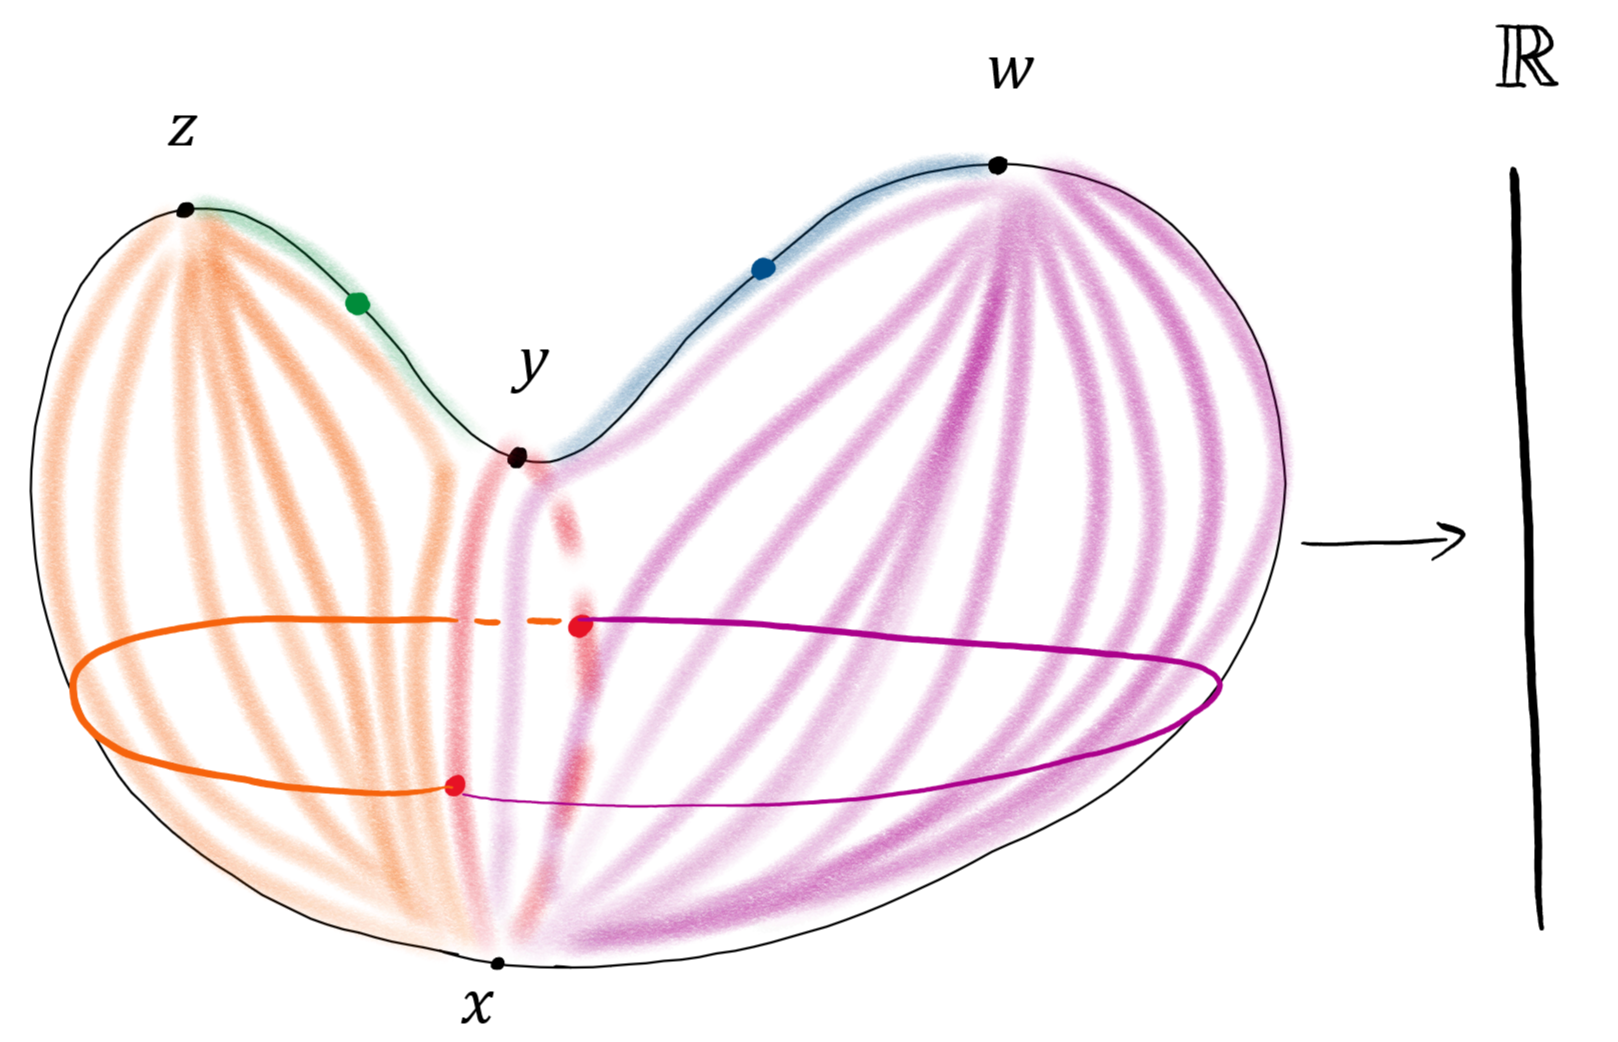
\includegraphics[scale=0.33]{fig/Heart.png}
\caption{A Smale-Morse function on the sphere, given as projection to the $z$ axis of the heart-shaped embedding. The letters represent critical points (with indices 2,2,1,0), the flow lines are drawn as soft, colorful lines, the solid colorful dots are representatives for the zero-dimensional flow manifolds and the solid colorful lines are representatives for the one-dimensional flow manifolds (notice the boundary structure as broken flow lines)}\label{fig:Heart}
\end{figure}

The compactification is given by adding \emph{broken flow lines}, which are piecewise smooth curves that start at $y$ and end at $x$ and pass through other critical points. We get that the flow manifolds have a \emph{corner structure}
\begin{equation*}
    \partial \flowM(z,x) = \bigcup_{\ind(z) > \ind(y) > \ind(x)} \flowM(z,y) \times \flowM(y,x).
\end{equation*}

see \cref{fig:Heart}. The fact that $\flowM(y,x)$ is constructed form the transverse intersection of two discs (one for curves ascending to $y$ and one for curves descending to $x$) gives a stable \emph{framing} on $\flowM(y,x)$ - a trivialization of the form 
\begin{equation*}
    T\flowM(y,x) \oplus \underline{\bbR}^{\ell_1} \overset{}{\simeq} \underline{\bbR}^{\ell_2}
\end{equation*}
where $\underline{\bbR}^{\ell_i}$ are trivial vector bundles over $\flowM(y,x)$. Moreover, the framing of all the flow manifolds is compatible with the corners structure.

\textbf{Morse homology}. It's worth saying that this data is sufficient to calculate the homology $H_*(M,\bbZ)$. It is given as the homology of the Morse chain complex $(C_*, d)$. The generators of $C_p$ are critical points with index $p$. Given two critical points $y,x$ with $\ind(y) -1 = \ind(x)$, the flow manifold $\flowM(y,x)$ is in fact compact; the coefficient of $x$ in $d(y)$ is given by the signed count of $\flowM(y,x)$, where the signs are determined by the framing. The boundary structure of the one-dimensional moduli spaces $\flowM(z, x)$ shows that $d^2 = 0$. See \cite{schwarz1993morse}.

\textbf{Bordism and generalized homology}. The fact that the flow manifolds are framed hints at an important theorem in differential topology, the Pontryagin-Thom isomorphism. We say that two closed framed $n$-manifolds $M_1$ and $M_2$ are \emph{bordant} if there is a framed $(n+1)$-manifold $W$, with $\partial W = M_1 \sqcup M_2$, in a way that is compatible with the framing. We denote by $\Omega^{\fr}_n$ the set of $n$ dimensional framed manifolds up to bordism. In fact the collection $\Omega_*^{\fr}$ form a graded ring, by disjoint union and Cartesian product.

The \emph{Pontryagin-Thom isomorphism} states that there is an isomorphism
\begin{equation*}
    \Omega_n^{\fr} \simeq \colim_k [S^{n+k},S^k]
\end{equation*}
between bordism groups of framed manifolds and stable homotopy groups of spheres (see \cite{pontryagin1955smooth, thom1954quelques}). The right hand side is also known as the coefficient ring $\pi_n(\bbS)$, where $\bbS$ is the spectrum representing stable homotopy.
We can view the Morse chain complex as a chain complex with coefficient ring $\bbZ = \Omega_0^{\fr} = \bbS_{\leq 0}$ and the differential is given by multiplication by the 0 dimensional flow manifolds $\flowM(y,x)$.

\textbf{Floer theory} A related question is the analysis of real-valued functions on objects that are not finite-dimensional closed manifolds. Floer developed this idea in the 1980s, leading to what is now known as Floer theory.
In general, Floer's idea is to generate a chain complex in which the differentials are defined by 'counting solutions' to a moduli problem (see \cite{floer1987morse} for initial formulations of this idea). In this case, the outcome does not yield the homology of a manifold, and one may ask: \textit{Are Floer homology groups merely the shadow of a more structured object?}

\textbf{Flow categories}. The development of a framework to address these questions led Cohen, Jones, and Segal (CJS) in \cite{CJS95} to introduce \emph{framed flow categories}, which axiomatize the data extracted from a Smale-Morse function on a manifold. In short, a framed flow category $\fC$ consists of a set of objects (corresponding to critical points) with a grading function $\norm{-}$ (corresponding to the index). For two objects $y,x \in \fC$, the morphism space from $y$ to $x$ is an ($\norm{y}-\norm{x}-1)$-dimensional manifold with corners, denoted $\flowM_{y,x}$, equipped with a choice of trivialization of $T\flowM_{y,x} \oplus \underline{\bbR^k}$ for some $k$ (corresponding to the stable framing).
Moreover, the composition is given by identifying the faces in the following way:
\begin{equation*}
    \flowM_{z,y} \times \flowM_{y,x} \hookrightarrow \flowM_{z,x}.
\end{equation*}
See \cref{sec:FFCat} for definitions and details.

Another building block in the theory are \emph{flow modules}. Given a flow category $\fC$, a right flow module $W$ over $\fC$ consists of a collection of manifolds $\{W_x\}_{x\in \fC}$, together with corner structure maps \begin{equation*}
    W_y \times \flowM_{y,x} \hookrightarrow W_x.
\end{equation*}
A right flow module is of \emph{degree} $i$ if 
\begin{equation*}
    \dim W_x = i - \norm{x}
\end{equation*}
for each pair of objects $y$ and $x$ in $\fC$. See \cite{porcelli2024bordism} definition 4.6, 4.7.
By abuse of notation, we denote the collection of right modules of degree $i$ over $\fC$ 
\begin{equation*}
    [*[i],\fC].
\end{equation*}
Similarly, we can define left flow modules of degree $i$ to be collections of manifolds $\{V_x\}_{x \in \fC}$, together with corner structure maps
\begin{equation*}
    \flowM_{y,x} \times V_x \hookrightarrow V_y.
\end{equation*}
such that $\dim V_x = \norm{x} - i$. We denote the collection of left modules of degree $i$ over $\fC$ by 
\begin{equation*}
    [\fC, *[i]].
\end{equation*}
A useful example for left module on a category $\fC$ is given by fixing $x' \in \fC$ and taking the collection
\begin{equation}
    \{\flowM_{x,x'}\}_{x \in \fC}.
\end{equation}
Indeed we have that the corner structure is given by the maps
\begin{equation*}
    \flowM_{y,x} \times \flowM_{x,x'} \hookrightarrow \flowM_{y,x'} 
\end{equation*}
The degree of this module is given by
\begin{equation*}
    \norm{x} - \dim (V_x) = \norm{x} - (\norm{x} - \norm{x'} - 1) = \norm{x'} + 1
\end{equation*}
and we denote is just by $\flowM_{-,x'}$.


\textbf{Filtrations and coherent chain complexes}. Another result of CJS was to attach a stable homotopy type to a framed flow category by the following idea.

Given a filtered space $X_0 \to X_1 \to \dots \to X_n = X$ we can take the successive cofibers to produce a ``chain complex" defined by
\begin{equation*}
    K_* \coloneq X_n/X_{n-1} \xrightarrow{d} \Sigma (X_{n-1}/X_{n-2}) \xrightarrow{d} \dots \xrightarrow{d} \Sigma^{n} X_0,
\end{equation*}
where $d^2$ is null-homotopic via the canonical null homotopy arising from $X$. Moreover, viewing $K_*$ from higher-categorical perspective allows us to encode additional data. In particular, there exist two null homotopies for $d^3$ that can be concatenated to form a loop in a suitable mapping space; the chain complex is then equipped with a null homotopy of this loop, and so forth. We call this structure a \emph{coherent chain complex}.
We can attempt to recover $X$ by taking \emph{iterated cofibers}. For example, note that
\begin{equation*}
    \S^2 X_1 = \cof \left (\S^1 X_1/X_0 \to \S^2 X_0 \right ), \quad \S^2 X_2 = \cof \left (\cof (X_2 / X_1 \to \S X_1/X_0) \to \S^2 X_0 \right )
\end{equation*}
and indeed, we can recover $X$ up to a certain suspension. See \cref{subsec:Ch&fil} and \cite{Ari21} for full detailed text.

Building on this idea, CJS showed that a framed flow category $\fC$ can be collapsed,via a Pontryagin-Thom-type construction, into a coherent chain complex $K$ in Spectra. After taking iterated cofiber, we obtain a spectrum
\[
    \norm{\fC} \coloneq \lim_p \cof (\cof (\dots \cof (\cof (K_p \to K_{p-1}) \to K_{p-2}) \to \dots \to K_1) \to  K_0)
\]
which is called the \emph{realization}\labeltext{realization}{txt:real} of $\fC$.
\begin{rem*}
    Note that $\norm{\fC}$ depends on the choice of framing for the manifolds $M_{b,a}$.
\end{rem*}

\textbf{Example - Morse flow category}. To combine the ideas of framed flow categories and chain complexes, let $f: \Man \to \bbR$ be a manifold equipped with a Smale-Morse function. First, we construct from $f$ a framed flow category $\fC_f$ - by taking $\flowM_{y,x} \coloneq \flowM(y,x)$, then we collapse it to a chain complex $K_{\fC_f}$ and realize it as $\norm{\fC_f} \in \Sp$. A result by CJS \cite{CJS95}, states that this procedure recovers the stable homotopy type of $M$:
\begin{equation*}
    \norm{\fC_f} \simeq \Sinf \Man.
\end{equation*}

This framework has proven useful in Floer theory, where the solutions to the moduli problem sometimes exhibit the structure of a flow category $\fC$. In such cases, we can realize the flow category, demonstrating that Floer homology is indeed a shadow of $\norm{\fC}$.

Looking back to Morse homology, we observe that the homology of a flow category can be determined from its zero-dimensional morphism manifolds. The fact that we can recover the stable homotopy type of $\Man$ from its framed flow category motivates the idea that we can read off the (generalized) homology of $\Man$ using the flow manifolds.

This idea goes back to Floer, who pointed out in \cite{floer1989witten} that: If $h_*$ is a general homology theory, trajectory space analysis suggests contributions from compact components of $\flowM(x, y)$. For stable homotopy $h_* = \pi^{s}_*$, this corresponds to the framed cobordism type. While higher-dimensional components of $\flowM(x, y)$ may not be compact, a modified approach could yield a spectral sequence. This framework has limited use in finite-dimensional Morse theory but may apply to infinite-dimensional settings. 


\todo{remove this "intuitive conclusion of introduction"?}\textbf{Gluing it together.} \emph{In this paper, given a flow category, we use the framework of CJS, Lurie, and Ariotta-Krause to generalize Floer’s idea and construct an Atiyah-Hirzebruch-like spectral sequence. This spectral sequence is given explicitly by gluing the flow manifolds.}

One can think of this result as the generalization of Morse and Floer homology in the sense that we provide a recipe for starting with a manifold or Floer data and reading off its generalized homology groups using the geometric and analytic data.

\subsection*{Notations}
We denote by $\Top$ the $1$-category of topological spaces, by $\Spaces$ the category of homotopy types (or $\infty$-groupoids), and $\Sp$ is the category of spectra. The stabilization functor is denoted $\Sinf: \Spaces \to \Sp$, and $\Ch(\Sp)$ and $\Fil(\Sp)$ denote the categories of coherent chain complexes in Spectra and (complete) filtered Spectra, respectively.

For a topological space $Y$, we denote by $Y_+$ its one-point compactification (if $Y$ is compact, then $Y_+ = Y \cup \{*\}$).
For a CW complex $Y$, we denote by $\sk_n Y$ its $n$-th skeleton.

For a stable tangential structure $\xi: \cX \to BO$, we denote by $\Omega^{\cX}_*$ the graded $\cX$-bordism ring and by $M\cX$ the Thom spectrum associated with the $\cX$-structure (see \cref{sec:tangStr} for definitions).

In this paper, a manifold is assumed to be a \emph{closed manifold} unless stated otherwise.

Let $\fC$ be a flow category. For $q,p \in \bbZ$ we denote by $\fC_{[q,p]}$ the full subcategory of $\fC$ consisting of objects satisfying $q \ge \norm{x}\ge p$, and we define $\fC_p \coloneqq \fC_{[p,p]}$. For brevity, we write 
\begin{equation*}
    M_{p,q}\coloneqq \bigsqcup_{y \in \fC_q, x \in \fC_p} M_{y,x}.
\end{equation*}
for the union of the flow manifolds, and for a right / left module over $\fC$ we write
\begin{equation*}
    W_p \coloneqq \bigsqcup_{x \in \fC_p} W_x, \quad V_p \coloneqq \bigsqcup_{x \in \fC_p} V_x.
\end{equation*}

Moreover, for a stable tangential structure $\xi: \cX \to BO$, one can define $\cX$ flow categories as those flow categories in which the morphism manifolds are equipped with an $\cX$ structure that is compatible with composition (in place of a stable framing). For an $\cX$ flow category $\fC$, we obtain a coherent chain complex $K_{\fC} \in \Ch(\Mod_{M\cX})$, and, analogously to the realization in $\Sp$ (see \ref{txt:real}), we define $\norm{\fC} \in \Mod_{\cX}$ to be its iterated cofiber.

\subsection*{Our results}
\label{def:Xrnp-extension}\todo{add begin defn?}
Let $\cX$ be a stable tangential structure, let $\fC$ be a $\cX$-structured flow category.
Let $n,p,r \in \bbZ$ and let $W,V$ be a right and left flow module over $\fC$ of degree $n$ and $p-r$ respectively. We define the punctured cube diagram
\begin{equation*}
    D: \ P(\{p,\dots,p-r\}) \setminus \{\varnothing\} \to \Top,
\end{equation*}
where $P(-)$ denote the power set, by setting
\begin{equation*}
    D(\{a_k, \dots, a_1\}) = W_{a_k} \times \flowM_{a_k,a_{k-1}} \times \flowM_{a_{k-1},a_{k-2}} \dots \times \flowM_{a_2,a_1} \times V_{a_1},
\end{equation*}
where $a_k > a_{k-1} > \dots > a_1$.
The \textbf{Toda manifold} is the colimit which we denote
\begin{equation*}
    V \circ W \coloneqq \colim D 
\end{equation*}
and we will see later that the Toda manifolds indeed have a manifold structure, and that they are closed, $(n-p+r)$-dimensional, $\cX$-structured.

For the spectral sequence, we consider a family of such constructions indexed by objects in $\fC_{p-(r+1)}$. Specifically, for each $z \in \fC_{p-(r+1)}$, we define a punctured cube diagram $D_z$ by replacing the left module $V$ with $\flowM_{-,z}$ in the general construction. This yields a Toda manifold
\begin{equation*}
    \flowM_{-,z} \circ W := \colim D_z \in \Omega^{\cX}_{n-p+r}.
\end{equation*}
Taking the disjoint union over all $z \in \fC_{p-(r+1)}$, we obtain an element
\begin{equation*}
    \bigsqcup_{z \in \fC_{p-(r+1)}} (\flowM_{-,z} \circ W) \in \bigoplus_{z \in \fC_{p-(r+1)}} \Omega^{\cX}_{n-p+r}.
\end{equation*}

\begin{exmp*}
    In \cref{fig:ffCat}, \ref{fig:k-boundary}, and \ref{fig:differential}, we can see an example of an extension and its Toda manifold.
\end{exmp*}

\begin{figure}[h!]
\[
\input{fig/rightLeftBimod Alt.tex}
\]
\caption{
The solid part represents the flow category $\fC$. Its objects are the $x_i$'s with $\norm{x_i}=i$, and the arrows represent the morphism manifolds.
The 0 dimensional framed manifold $w_4$ represents an element in $E_1^{4,4} = \Omega^{\fr}_{4-4}$.
The dashed arrows represent an right module over $\fC_{[4,2]}$.
The symbols $\pm$, $I$, etc., represent the flow manifolds themselves (where $\pm$ represents a framed point; the rest of framing is omitted for clarity).
}\label{fig:ffCat}
\end{figure}

\captionsetup{font={small}}
\begin{figure}[h!]
\centering
\begin{minipage}{.61\textwidth}
  \centering
  \adjustbox{width=\linewidth}{\begin{tikzcd}
{W_4\times M_{4,3}\times M_{3,2}\times M_{2,1}} && |[myyellow]|{W_4\times M_{4,3}\times M_{3,1}}& \\
\\
& |[mygreen]|{W_4\times M_{4,2}\times M_{2,1}} && |[myviolet]|{W_4\times M_{4,1}} \\
\\
|[myred]|{W_3\times M_{3,2}\times M_{2,1}} && {\textcolor{myred}{W_3} \times \textcolor{myyellow}{M_{3,1}}} \\
\\
& |[myblue]|{W_2\times M_{2,1}}
\arrow[gray,from=1-1, to=1-3]
\arrow[gray,from=1-1, to=3-2]
\arrow[gray,from=1-1, to=5-1]
\arrow[gray,from=1-3, to=3-4]
\arrow[gray,from=1-3, to=5-3]
\arrow[gray,from=5-1, to=5-3]
\arrow[gray,from=5-1, to=7-2]
\arrow[gray,from=3-2, to=7-2, crossing over]
\arrow[gray,from=3-2, to=3-4, crossing over]
\end{tikzcd}}
  \captionof{figure}{
  the \cref{fig:ffCat} (from $*$ to $x_2$) and the\\object $*$ construct the punctured cube $D_{*}$
  }
  \label{fig:k-boundary}
\end{minipage}\hfill
\begin{minipage}{.37\textwidth}
  \centering
  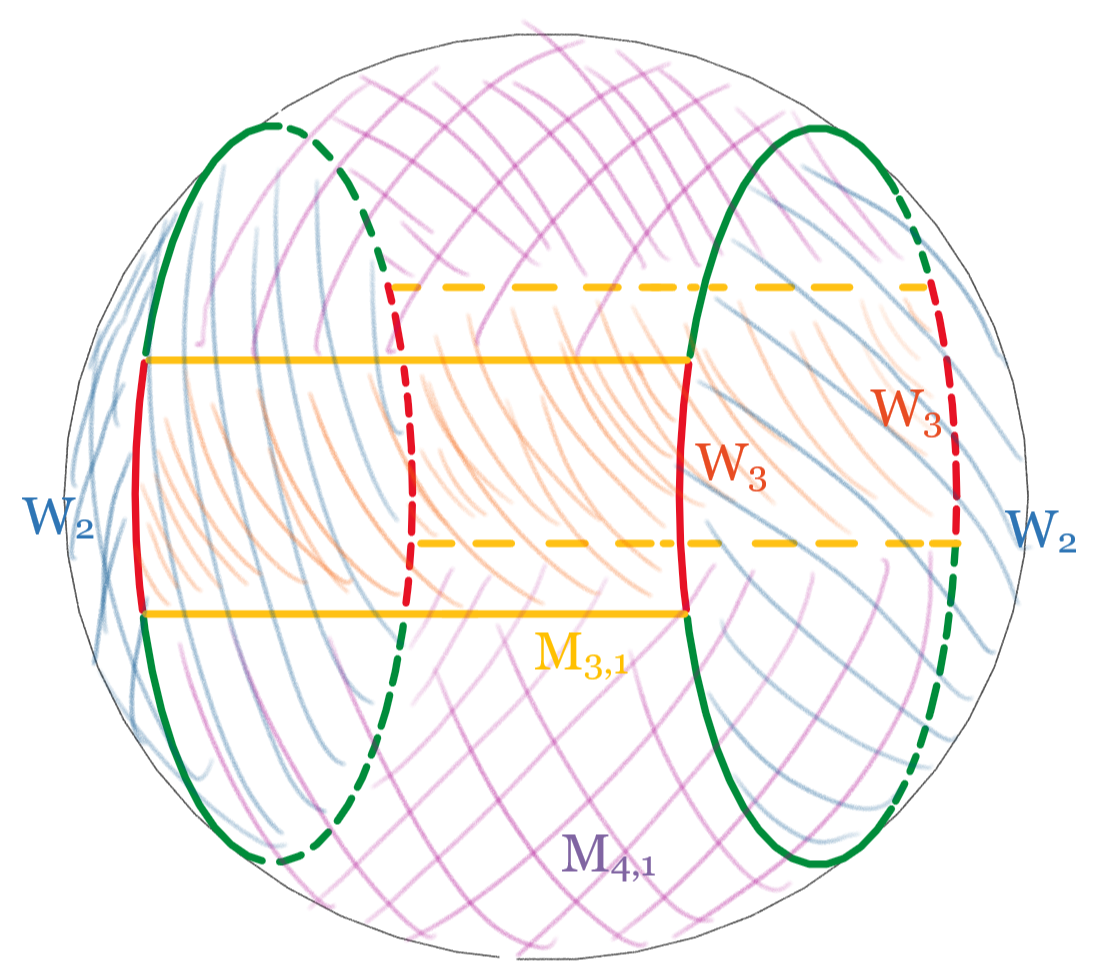
\includegraphics[width=\linewidth]{fig/Toda Manifold drawing - with M labels.png}
  \captionof{figure}{
  We can see that $\colim D_{*}$ is a topological space that inherits a closed smooth manifold structure.
  }
  \label{fig:differential}
\end{minipage}
\end{figure}

\newpage
\begin{restatable}{thmA}{ThA}\label{SSofStrFFCat}
    Let $\fC$ be a flow category with an $\cX$-tangential structure. There is a spectral sequence:
    \begin{equation*}
        \pg{E}{1}{n}{p} = \bigoplus_{\norm{z}=p} \Omega^{\cX}_{n-p}
    \end{equation*}
    which converges to the homotopy groups of the realization:
    \begin{equation*}
        \rnp{E} \implies \pi_n \norm{\fC}.
    \end{equation*}
    An element $W_p=\{W_z\} \in \pg{E}{1}{n}{p}$ survives to $\pg{E}{r+1}{n}{p}$ if and only if we can extend the collection $W_p$ to an right flow module, over $\fC_{[p,p-r]}$. The differential is represented geometrically by the Toda manifolds:
    \begin{equation*}
        d_{r+1}(W_p) = \{\flowM_{-,z} \circ W\}_{z \in \fC_{p-(r+1)}} \in \bigoplus_{z \in \fC_{p-(r+1)}} \Omega^{\cX}_{n-p+r} = \pg{E}{r+1}{n-1}{p-(r+1)}
    \end{equation*}\todo{write as $\bigcup$}
\end{restatable}

A key tool used to prove \cref{SSofStrFFCat} is a description of the spectral sequence associated with a coherent chain complex expressed in terms of chain complex maps.

\begin{restatable}{thmA}{ThB}\label{SSofCh}
    Let $K \in \Ch(\Sp)$ be a coherent chain complex in Spectra. Then there is a spectral sequence:
    \begin{equation*}
        E_1^{n,p} = \pi_{n - p} K_p,
    \end{equation*}
    which converges to
    \begin{equation*}
        E_r^{n,p} \implies \pi_n \colim_p (\cI K)_p,
    \end{equation*}
    
    Moreover, let $x: \mathbb{S}^{n - p} \to K_p$ represent an element of $\pg{E}{1}{n}{p}$. Then $x$ survives to $\pg{E}{r+1}{n}{p}$ if and only if there exists a chain map:
    \begin{equation}\label{eq:x_ext}
        \xymatrix{
        \mathbb{S}^{n - p} \ar[d]_{x} \ar[r] & 0 \ar[r]\ar[d] & \dots \ar[r]\ar[d]& 0\ar[d]\\
        K_p \ar[r]^{d_p}& K_{p - 1} \ar[r]^{d_{p - 1}}& \dots \ar[r]^{d_{p - r} \quad}& K_{p - r}
        }
    \end{equation}
    Here, the top row is concentrated in degree $p$, and the bottom row is the restriction of $K$ from degree $p$ down to $p-r$.
    The differential $\partial_{r+1}(x)$ is given by the composition of chain maps:
    \begin{equation*}
        \xymatrix
        {   \mathbb{S}^{n-p} \ar[r]\ar[d]_x & \dots \ar[r]\ar[d] &  0 \ar[d]\\
            K_p \ar[r]\ar[d] & \dots \ar[r]\ar[d] &  K_{p-r} \ar[d] \\
            0 \ar[r] & \dots \ar[r] & K_{p-r-1} 
        }
    \end{equation*}
    The first map is precisely \cref{eq:x_ext} and the second is induced by the structure of the chain complex $K$.
\end{restatable}
We obtain this result by combining the description of the spectral sequence of a filtered object in Lurie \cite{Lur17} with the results of~\cite{Ari21}.

\subsection*{Relation to other work}\todo{Delete everything which is not directly related to flow categories (delete all the Khovanov, Arnold, knots,...)}
This paper contributes to the broader project of providing a geometric model for spectra. For the foundation of this project, which defines the stable $\infty$-category of framed flow categories and establishes its equivalence with the category of spectra, see \cite{abouzaid2024foundation}.

This project traces back to the work of Cohen-Jones-Segal (CJS) in \cite{CJS95}, where the term “flow category” was introduced as a means of organizing the data of a Morse-Smale function in a categorical way. In that work, a coherent version of chain complexes is constructed from such a category, and these chains are subsequently “realized” as a filtered spectrum. These ideas have since proven very useful in Floer theory.

In knot theory, organizing the data of knots into a flow category results in a stable homotopy type that lifts Khovanov homology (see \cite{LS14}). Moreover, by simplifying the flow categories (see \cite{lobb2018framed, lobb2017calculus}) and classifying $0$- and $1$-dimensional manifolds, one obtains a combinatorial description and an effective algorithm for computing the operations
\[
    \operatorname{Sq}^2 : H^\ast(\fC, \mathbb{Z}/2) \to H^{\ast+2}(\fC, \mathbb{Z}/2)
\]
from a knot diagram. This leads to the calculation of the corresponding homotopy (see \cite{lobb2020khovanov, lipshitz2014steenrod}). For a recap of flow categories in Khovanov and knot Floer theories, see \cite{marengon2024spectra}.

Our work is similar in spirit to these developments in that we use higher flow manifolds to compute the differentials, which can be interpreted as higher cohomology operations.

In Hamiltonian Floer theory, one of the breakthroughs related to the Arnold conjecture employed a CJS-like construction—a generalization of flow categories adapted to Hamiltonian flow data—to prove a version of the Arnold conjecture over a field of characteristic $p$ (see \cite{abouzaid2021arnold}). Similar ideas appear in the work on the integral Arnold conjecture (see \cite{rezchikov2022integral, bai2022arnold}). Another recent development is the theory of Morse-Bott flow categories, where the function has critical sets (rather than isolated points) (see \cite{bonciocat2024revisiting}). An ongoing line of research is the introduction of an equivariant structure on such categories, which in turn induces an equivariant structure on the realization spectrum—a framework that supports cyclotomic methods in symplectic geometry (see \cite{cote2023equivariant, rezchikov2024cyclotomic}).

One also finds flow-category-like constructions in Lagrangian geometry that lift the Fukaya category of a symplectic manifold (see \cite{porcelli2024bordism, porcelli2024spectral}).

\begin{rem}
    In this paper we treat flow categories as chain complexes in $\Sp$ or, equivalently, as filtered spectra. We expect that there is a construction analogous to that in \cite{abouzaid2024foundation} which provides a flow-categorical model for $\{K_p\} \in \Ch(\Sp)$ such that $K_p = \bigoplus \mathbb{S}$.
\end{rem}

The interpretation of gluing manifolds as Toda brackets or Massey products appears in \cite{alexander1972cobordism}, where the Massey product is defined via the gluing of two manifolds with boundary.

\Cref{SSofCh} bears a similar flavor to other works on spectral sequences associated with various objects. In \cite{Ari21}, the authors explain the connection between filtered objects and coherent chain complexes, and they also define a spectral sequence for coherent chain complexes using the Beilinson $t$-structure. We also recommend \cite{antieau2024spectral} as an introduction to spectral sequences and their relation both to chain complexes and to the spectral sequence of filtered objects defined in \cite{Lur17}. The construction of the spectral sequence in this paper is similar to that in \cite{blanc2022spectral}, where the authors define a spectral sequence associated with a simplicial object.

\subsection*{Paper layout}
Section~2 is devoted to the framework of chain complexes in (stable) $\infty$-categories and contains the proof of \Cref{SSofCh}.

In Section~3, we recall the definitions of manifolds with corners, framed flow categories, and the Pontryagin-Thom construction for manifolds with corners. At the end of this section, we demonstrate several properties of the Pontryagin-Thom construction that will be useful in later sections.

Section~4 establishes a correspondence between chain complexes in the category of spectra (with values $\bigoplus \mathbb{S}$) and framed flow categories.

Our goal in Sections~5 and~6 is to upgrade this correspondence so that it interacts naturally with spectral sequences. In other words, given a framed flow category, we show how to produce a spectral sequence for the corresponding chain complex and provide a geometrical description of its pages and differentials.

In Section~5, we compare various models for chain complexes by considering different models for $\infty$-categories (namely, topologically enriched, simplicially enriched, and simplicial sets). This comparison allows us to give a straightforward description of the composition of maps between flow categories.

Section~6 translates this description of composition into a geometrical framework and establishes the existence of a spectral sequence associated with framed flow categories.

In the final section, we explain how the framing structure can be replaced by a more general tangential structure, and we discuss how different structures interact. This section also contains examples of spectral sequences arising from flow categories.

\subsection*{Discussion and open problems}
\textbf{Different definitions for flow categories.} In \cite{abouzaid2024foundation}, the authors construct an $\infty$-category $\mathrm{Flow}^{\fr}$ (see also \cite{porcelli2024bordism} for the homotopy category) and show that it is equivalent to $\Sp$. We now explain the main difference between their work and ours from an algebro-topological perspective. Let $M$ be a compact manifold. Given two Morse-Smale functions $f$ and $g$, one obtains two framed flow categories, $\fC_f$ and $\fC_g$. By interpolating between $f$ and $g$, we obtain two maps in $\mathrm{Flow}^{\fr}$
\[
    H_{f,g}: \fC_f \to \fC_g, \quad H_{g,f}: \fC_g \to \fC_f,
\]
and by homotoping the compositions we obtain 2-morphisms
\[
    H_{g,f} \circ H_{f,g} \simeq \mathrm{Id}, \quad H_{f,g} \circ H_{g,f} \simeq \mathrm{Id}.
\]
Hence, the flow category of $M$ is independent of the choice of Morse-Smale function.

On the other hand, the functions $f$ and $g$ induce CW structures on $M$, and different CW structures yield different (Atiyah-Hirzebruch) spectral sequences. Therefore, one cannot define a spectral sequence as an invariant of the equivalence classes in $\mathrm{Flow}^{\fr}$.

To address this issue, we conjecture that one can define another $\infty$-category, with a modified class of morphisms. Specifically, for a 2-morphism $R$ between flow categories $\fC$ and $\sD$, and for objects $x \in \fC$ and $y \in \sD$, we require that if $\|y\| > \|x\|$, then $R_{x,y} = \varnothing$ (rather than being a manifold of dimension $\|y\| - \|x\|$). This construction should yield a subcategory of $\Fil(\Sp)$ in which the two Morse-Smale functions on a manifold $M$ produce distinct objects.

Using this perspective, we can think of \cref{SSofStrFFCat} as a spectral sequence of filtered flow category $F \in \Fil(\mathrm{Flow}^{\cX})$ where the filtration is induces by the index filtration on a flow category.

In this paper the full $\infty$-categorical structure is unnecessary; instead, we define the equivalence relation on flow categories by pulling it back from the category $\Ch(\Sp)$ (see \Cref{prop:FF_are_Ch}).
\subsection*{Acknowledgments}
I am grateful to my advisor, Tomer Schlank, for introducing me to the ideas behind this paper, for guiding me toward this project, and for fostering a great research environment. I am also grateful to the Seminarak group, particularly Shai Keidar and Shaul Ragmov, for insightful discussions over time, and to Lior Yanovski for his efforts in maintaining the group in recent months. I would like to thank Trygve Poppe Oldervoll, João Lobo Fernandes, and David Blanc for their comments and suggestions. Finally, I sincerely appreciate Shulamit’s support and Edo and Orit’s hospitality during the writing of this paper.

This project was partially supported by ISF grant 437/20.
\newpage

\section{Chains Complexes and their Spectral Sequences}\label{sec:Ch}
Spectral sequences for filtered objects in Spectra are treated in Lurie's work \cite{Lur17}. A key insight, developed by Ariotta and Krause \cite{Ari21}, is that within a stable $\infty$-category, filtered objects are equivalent to coherent chain complexes. Building upon this equivalence, this section aims to provide an explicit description of the spectral sequence associated with a coherent chain complex.

\subsection{Chain Complexes and Filtered Objects} \label{subsec:Ch&fil}
In this section, let $\cC$ be a stable $\infty$-category with sequential limits and colimits.
Following \cite{Ari21}, we will introduce the categories of chain complexes and filtered objects in $\infty$-category. We will show how to connect between them and the equivalence between the two categories.

\begin{rem}
    For being compatible with flow categories, our chain complexes will decrease and hence the filtered objects will increase, as oppose to \cite{Ari21}. 
\end{rem}

\begin{defn}\label{def:Ch}
    We define the category $\Ch$ to be the pointed (ordinary) category with
    \begin{equation*}
        \ob \ \Ch \coloneqq \mathbb{Z} \cup \{*\}
    \end{equation*}
    \begin{equation*}
        \Hom_{\Ch}(i,j) \coloneqq \begin{cases}
            \{ \mathrm{id}, \zeroMor \} & i=j \\
            \{ d_i, \zeroMor \} & i=j+1 \\
            \{\zeroMor\} & \text{otherwise}
        \end{cases}
    \end{equation*}
    where $*$ is the zero object and $\zeroMor$ is the map $i \to * \to j$.

    For $\cC$ as above, we define \textit{chain complexes in $\cC$} (or just \textit{chains}) to be the full subcategory
    \begin{equation*}
        \Ch(\cC) \coloneqq \Fun^*(\Ch,\cC) \subset \Fun(\Ch,\cC)
    \end{equation*}
    of pointed functors.

    We denote by $\Chb$ the full subcategory of $\Ch(\cC)$ spanned by the objects $K$ such that there exists $N \in \mathbb{N}$ with:
    \begin{equation*}
        K_i = \zr \text{ for all } i < N.
    \end{equation*}
    We call such chain complexes \emph{bounded below}.
\end{defn}

\begin{rem*}
    If we don't mention otherwise, we assume that $K \in \Chb$ is bounded below by $N=0$.
\end{rem*}

\begin{exmp*}
    The category $\Ch(\Ab)$ of chain complexes in abelian groups is the usual category of chain complexes.
\end{exmp*}
\begin{rem}\label{rem:higher_ch}
    In the case where $\cC$ is an $\infty$-category, the reader may want to think of $\Ch(\cC)$ as chain complexes, with null-homotopies of the composition of two maps along with higher null-homotopies: given a composition of three maps in the chain complex
    \begin{equation*}
        K_p \to K_{p-1} \to K_{p-2} \to K_{p-3},
    \end{equation*}
    we get two null-homotopies of the map $K_p \to K_{p-3}$, which give us a map $S^1 \to \Hom(K_p,K_{p-3})$. Part of the data of a chain complex is a null-homotopy of this loop and similarly higher null-homotopies for higher loops.
\end{rem}

\begin{defn}
    We denote by $\mathbb{Z}$ the category of integers with the usual increasing order.
\end{defn}

\begin{defn}
    Let $\cC$ be a stable $\infty$-category with sequential limits and colimits. We define the category of (increasing, complete) \emph{filtered objects in $\cC$} to be the full subcategory
    \begin{equation*}
        \Fil(\cC) \subset \Fun(\mathbb{Z},\cC)
    \end{equation*}
    spanned by functors $F$ such that $\lim_p F_p = \zr$; sometimes denoted by $\widehat{\Fil}(\cC)$. We define the \textbf{bounded below filtered objects} to be the full subcategory
    \begin{equation*}
        \Filb(\cC) \subset \Fil(\cC)
    \end{equation*}
    spanned by functors $F$ such that there exists $N \in \mathbb{N}$ with $F_p = \zr$ for $p < N$.
\end{defn}

Note that the image of the stable Yoneda embedding
\begin{equation*}
    \yo_{(-)}: \bbZ^{\Op} \to \Fun(\bbZ, \Sp) = \Fil(\Sp).
\end{equation*}
is given by
\begin{equation*}
    \yo_p(q) = \Map_{\Sp}(p,q) = \begin{cases}
        \bbS & q \geq p \\
        0 & q < p
    \end{cases}
\end{equation*}
Let $p \to (p-1)$ be a morphism in $\bbZ^{\Op}$, the morphisms $\yo_p \to \yo_{p-1}$ is given by
\begin{equation*}
    \xymatrix{
        \dots \ar[r] & 0 \ar[r]\ar[d] & 0    \ar[r]\ar[d]    & \bbS \ar[d]\ar[r]   & \dots \\
        \dots \ar[r]        & 0 \ar[r]       & \bbS \ar[r]          & \bbS \ar[r]         & \dots
    }
\end{equation*}

\begin{defn}\label{def:lacunarCh}
    For $n,p \in \bbZ$ we define the following chain complex $\bbS_p^{n} \in \Ch(\Sp)$ by
    \begin{equation*}
        \bbS_p^{n}(q) \coloneqq \begin{cases}
            \bbS^n & q = p \\
            0 & \text{otherwise}
        \end{cases}
    \end{equation*}
\end{defn}
Note that there is the map in $\Ch(\Sp)$
\begin{equation*}
    Y_{n,p} \colon \bbS^{n-1}_{p} \to \bbS^n_{p-1}
\end{equation*}
which visually  given by
\begin{equation*}
    \xymatrix{
        \dots  \ar[r] & 0 \ar[r]\ar[d] & \bbS^{n-1}    \ar[r]\ar[d]    & 0 \ar[d]\ar[r]   & 0 \ar[d]\ar[r] & \dots\\
        \dots \ar[r]        & 0 \ar[r]       & 0 \ar[r]                & \bbS^n \ar[r]    & 0 \ar[r]        & \dots
    }
\end{equation*}
which is defined using the fact that $\bbS^n \simeq \S \bbS^{n-1}$ in $\Sp$.

In particular we have a map
\begin{equation*}
    Y_p \coloneqq Y_{-(p-1),p}\colon \bbS^{-p}_{p} \to \bbS^{-(p-1)}_{p-1}
\end{equation*}

\begin{defn}
    We define 
    \begin{equation*}
        \cA \colon \Fil(\Sp) \to \Ch(\Sp)
    \end{equation*}
    to be the colimit preserving functor that determined by mapping
    \begin{equation*}
        \cA (\yo_p) \coloneqq \bbS^{-p}_p
    \end{equation*}
    and the morphisms are given by $Y_p$.
    
    We denote it's right adjoint 
    \begin{equation*}
        \Fil(\Sp) \leftarrow \Ch(\Sp) \colon \cI
    \end{equation*}
\end{defn}

In \cite{Ari21}, Ariotta define these functors and proves
\begin{thm}[\cite{Ari21}]\label{th:Ch_Fil_eq}
    Let $\cC$ be a stable $\infty$-category with sequential limits and colimits. We have an equivalence
    \begin{equation*}
        \cA: \Fil(\cC) \simeq \Ch(\cC) : \cI.
    \end{equation*}
\end{thm}
An immediate consequence is the representability of the evaluation:
\begin{equation}\label{eq:F_p_is_rep}
    \Map(\bbS^{-p}_p, \cA F) \simeq \Map(\cI \bbS^{-p}_p, F) \simeq \Map(\yo_p, F) \simeq F_p
\end{equation}

\begin{defn}
    Let $\cC$ be a stable $\infty$-category and $p \in \bbZ$, we write $\iota_{[p-1,p]}: \{(p-1) \to p\} \to \mathbb{Z}$ for the inclusion functor and
    \begin{equation*}
        (\iota_{[p-1,p]})^*: \Fun(\mathbb{Z},\cC) \to \Fun(\Delta^1,\cC)
    \end{equation*}
    for the restriction (pre-composition) along $\iota_{[p-1,p]}$. We define the $p$-th associated graded functor by:
    \begin{equation*}
        \gr_p \coloneqq \cof \circ (\iota_{[p-1,p]})^* : \Fun(\mathbb{Z},\cC) \to \cC,
    \end{equation*}
    so that
    \begin{equation*}
        F \mapsto F_p/F_{p-1}.
    \end{equation*}
    The map
    \begin{equation*}
        F_p/F_{p-1} \to \Sigma F_{p-1}/F_{p-2}
    \end{equation*}
    given by the connecting morphism of the cofiber, and then taking quotient, induces a transformation:
    \begin{equation*}\label{eq:Fil_str_map}
        \gr_p \to \Sigma \gr_{p-1}.
    \end{equation*}
\end{defn}

A direct calculation shows that
\begin{equation*}
    \S^{-p} \gr_q(\yo_p) = (\cA \yo_p)_q
\end{equation*}
and we deduce that
\begin{cor}
    \begin{equation*}
        (\cA -)_p \simeq \S^{-p} \gr_p (-)
    \end{equation*}
    As functors 
    \begin{equation*}
        \Fil(\Sp) \to \Sp
    \end{equation*}
\end{cor}

We now provide an explicit expression for $\cI$.

First, we define a the following chain complex  in $\Sp$,
\begin{equation*}
    \S^{n}y_p \coloneqq \begin{cases}
        \bbS^{n} & q \in \{p,p-1\} \\
        0 & \text{otherwise}
    \end{cases}
\end{equation*}
In particular we have
\begin{equation*}
    \cof(Y_p) \simeq \S^{-(p-1)}y_p
\end{equation*}

On the other hand (see \cite{Ari21} Lemma 3.12), one can show that the evaluation functor
\begin{equation*}
    (-)_p \colon \Ch(\Sp) \to \Sp, \quad K \mapsto K_p
\end{equation*}
is represented:
\begin{equation*}
    \Map(y_p, -) \simeq (-)_p.
\end{equation*}
The objects in the following fiber sequence
\begin{equation}\label{req:RepFibSeq}
    \bbS^{-p}_{p} \to \bbS^{-(p-1)}_{p-1} \to \cof(Y_p)
\end{equation}
represents the functors
\begin{equation*}
    (\cI -)_p, \quad (\cI -)_{p-1}, \quad \S^{-(p-1)} (-)_p.
\end{equation*}
By taking the contravariant $\Map$ functor to \cref{req:RepFibSeq} we get the following result:
\begin{lem}\label{lem:calc_cI}
    There is a cofiber sequence of functors
    \begin{equation}
        \S^{-(p-1)} (-)_p \to (\cI -)_{p-1} \to (\cI -)_p
    \end{equation}
\end{lem}
A simple corollary is
\begin{cor}
    Let $K \in \Ch_b(\Sp)$ bounded below by $N$. Then for $p \le N$ we have
    \begin{equation*}
        (\cI K)_p = 0
    \end{equation*}
\end{cor}
which obtained by inductively applying \cref{lem:calc_cI}.


\begin{exmp*}
    Let
    \begin{equation*}
        \dotsb \to \zr \to F_0 \to F_1 \to F_2 \to F_3 \to 0 \to\dotsb
    \end{equation*}
    be a filtered object in $\Sp$. Then $K \coloneqq \cA F$ is given by:
    \begin{equation*}
        \dotsb \to \zr \to \Sigma^{-3} F_3/F_2 \to \Sigma^{-2} F_2/F_1 \to \Sigma^{-1} F_1/F_0 \to F_0 \to \zr \dotsb
    \end{equation*}
    where the zeros on the left are $F_3 / F_3$. The composition 
    \begin{equation*}
        K_3 = \Sigma^{-3} F_3/F_2 \to \Sigma^{-2} F_2/F_1 \to \Sigma^{-1} F_1/F_0 = K_1
    \end{equation*}
    can be factored as:
    \begin{equation*}
        \Sigma^{-3} F_3/F_2 \to \Sigma^{-2} F_2 \to \Sigma^{-2} F_2/F_1 \to \Sigma^{-1} F_1 \to \Sigma^{-1} F_1/F_0,
    \end{equation*}
    where the middle part is a cofiber sequence; hence, the composition is null-homotopic. Following \cref{rem:higher_ch}, this null-homotopy is the "non-higher" part of the chain complex $K$.

    To recover $F = \cI K$ from $K$, we can use \cref{lem:calc_cI}. The fact that $K$ is bounded below by $-1$ yields that
    \begin{equation*}
        (\cI K)_p = 0\quad \text{for $p \leq -1$}
    \end{equation*}
    From that following cofiber sequence We ca see that $F_0 = K_0$ 
    \begin{equation*}
        \S^{-(-1)}K_0 \to \overbrace{F_{-1}}^{=0} \to F_0.
    \end{equation*}
    We can recover $F_1$ as the cofiber
    \begin{equation*}
        K_1 \to \overbrace{F_0}^{=K_0} \to F_1.
    \end{equation*}
    And by taking $F_2$ is reconstructed as an iterated cofiber, from the cofiber sequence :
    \begin{equation*}
        \S^{-1} K_2 \to \overbrace{F_1}^{=K_1/K_0} \to F_2.
    \end{equation*}
\end{exmp*}

\begin{rem}\label{ex:CW_skl}
    An ''non example'' is given by taking a topological space $X$ and the filtered space $F_p \coloneq \sk_p X$.
    If $X$ is finite, then there is an $N \in \bbN$ - an upper bound for the filtration.
    In this case, we can define the following chain complex in $\Spaces$
    \begin{equation*}
        K_p \coloneqq \S^{N-p} \gr_p F= \sk_p X / \sk_{p-1} X \simeq \bigvee_{\text{p cells}} S^N
    \end{equation*}
    and the morphisms $\gr_p \to \Sigma \gr_{p-1}$ that induces the maps $K_p \to K_{p-1}$, are given by the maps:
    \begin{equation*}
        \WedgeSpaces S^p = \sk_p X / \sk_{p-1} X \xrightarrow{\partial_p} \sk_{p-1} X / \sk_{p-2} X = \Sigma \WedgeSpaces S^{p-1},
    \end{equation*}
    which are more commonly known as the differentials in the chain complex that computes the cellular homology of $X$.
    By taking iterated cofibers we can recover $F$ only up to suspension, for example
    \begin{equation*}
        \S^N F_1 \simeq \cof(\S^{N-1} F_1 /F_0 \to S^N F_0)
    \end{equation*}
\end{rem}

\subsection{Spectral Sequences of Chain Complexes}\label{sec:SSofCh}
We will start with the construction of spectral sequence of a filtered object, following the notations and definitions in \cite{Lur09}. Combined with the last subsection we will get a description of the pages of a spectral sequence of a chain complex. The main output is \cref{lem:ChSur}.

For our discussion, we assume that $\cC$ is a stable $\infty$ category equipped with a $t$-structure $(\cC^{\leq 0}, \cC^{\geq 0})$.
We begin by defining the spectral sequence associated with a filtered object in $\cC$.

\begin{defn}{\cite[Def.\ 1.2.2.9]{Lur17}}\label{def:SS_Fil}
Let $F$ be a filtered object in $\cC$, i.e., a sequence of morphisms $\{ F_p \}_{p\in \mathbb{Z}}$ such that
\begin{equation}
\cdots \to F_{p-1} \to F_p \to F_{p+1} \to \cdots.
\end{equation}
For each $p \in \mathbb{Z}$, define the graded pieces by
\begin{equation}
\gr_p F = \cofib(F_{p-1} \to F_p).
\end{equation}
We define a spectral sequence $\{ E_r^{n,p}, d_r^{n,p} \}$ associated with $F$ by setting
\begin{equation}\label{eq:Er_Fil}
E_r^{n,p} = \Image\left( \pi_n\left( \nicefrac{F_p}{F_{p - r}} \right) \to \pi_n\left( \nicefrac{F_{p + r - 1}}{F_{p - 1}} \right) \right),
\end{equation}
where the map is induced by the compositions of the inclusion and projection:
\begin{equation}\label{eq:factorization}
    \nicefrac{F_p}{F_{p - r}} \to \nicefrac{F_p}{F_{p - 1}} \to \nicefrac{F_{p + r - 1}}{F_{p - 1}}.
\end{equation}

The differentials $d_r^{n,p}\colon E_r^{n,p} \to E_r^{n-1, p - r}$ are determined by the connecting morphisms via the commutativity of the diagram:
\begin{equation}\label{eq:diff_Fil}
\xymatrix{
\pi_n\left( \nicefrac{F_p}{F_{p - r}} \right) \ar[r]\ar[d]^{\delta_{p - r}} & E_r^{n,p} \ar[r]\ar[d]^{d_r^{n,p}} & \pi_n\left( \nicefrac{F_{p + r - 1}}{F_{p - 1}} \right) \ar[d]^{\delta_{p - 1}}\\
\pi_{n - 1}\left( \nicefrac{F_{p - r}}{F_{p - 2r}} \right) \ar[r] & E_r^{n - 1, p - r} \ar[r] & \pi_{n - 1}\left( \nicefrac{F_{p - 1}}{F_{p - r - 1}} \right),
}
\end{equation}
where the vertical maps $\delta_{p - r}$ and $\delta_{p - 1}$ are the connecting homomorphisms from the long exact sequences of homotopy groups associated with the cofiber sequences:
\begin{equation}
F_{p - r} \to F_p \to \nicefrac{F_p}{F_{p - r}} \quad \text{and} \quad F_{p - 1} \to F_{p + r - 1} \to \nicefrac{F_{p + r - 1}}{F_{p - 1}}.
\end{equation}
\end{defn}

\begin{thm}{\cite[Prop.\ 1.2.2.14]{Lur17}}\label{th:converge}
Let $\cC$ be a stable $\infty$-category equipped with a t-structure, that admits sequential colimits and that the t-
structure is compatible with sequential colimits. Let $F$ be a complete filtered object in $\cC$. Then the spectral sequence $\{ E_r^{n,p}, d_r^{n,p} \}$ (see \cref{def:SS_Fil}) converges to the homotopy groups of the colimit of $F$:
\begin{equation*}
E_r^{n,p} \Rightarrow \pi_n \colim_p F_p.
\end{equation*}
\end{thm}

\begin{exmp}\label{ex:CW_pages}
Consider a CW complex $X$ with its skeletal filtration $\{ \sk_p X \}_{p \geq 0}$. Applying the suspension spectrum functor $\Sigma^\infty$, we obtain a filtered spectrum $F$ in $\Sp$, where $F_p = \Sigma^\infty \sk_p X$. Let $K = \cA F$ be the associated chain complex (as in \cref{ex:CW_skl}). The spectral sequence arising from this filtration has first page:
\begin{equation*}
E_1^{n,p} = \pi_n \gr_p F = \pi_n \left( \WedgeSp \mathbb{S}^p \right) = \pi_{n - p} K_p,
\end{equation*}
since each $\gr_p F$ is a wedge of spheres suspended $p$ times, and $K_p$ is the $p$-th term in the chain complex $K$.

This spectral sequence converges to:
\begin{equation*}
\pi_n \Sigma^\infty X,
\end{equation*}
which are the stable homotopy groups of the space $X$.

More generally, for any spectrum $A$, we can consider the filtered spectrum $F_p \otimes A$, obtaining a spectral sequence converging to the generalized homology:
\begin{equation*}
A_n(X).
\end{equation*}
This spectral sequence is known as the \emph{Atiyah--Hirzebruch spectral sequence}.
\end{exmp}

\begin{defn}\label{def:survive}
Let $F$ be a filtered object in stable $\infty$-category $\cC$ and let $\rnp{E}$ be it's spectral sequence. An element $x \in E_1^{n,p}$ is said to \textbf{survive to the $r$-th page} if it lies in the image of the map:
\begin{equation*}
x \in \Image \left( \pi_n\left( \nicefrac{F_p}{F_{p - r}} \right) \to \pi_n\left( \nicefrac{F_p}{F_{p - 1}} \right) \right).
\end{equation*}
We denote the collection of such elements by $\mathcal{E}_r^{n,p}$. If $x' \in \pi_n\left( \nicefrac{F_p}{F_{p - r}} \right)$ maps to $x$, we say that $x'$ \textbf{lifts} $x$.
\end{defn}

Intuitively, an element survives to the $r$-th page if it is not killed by the differentials $d_k$ for $1 \leq k < r$.

\begin{rem}\label{rem:FirstPageDesc}
In the stable homotopy category $\Sp$, the homotopy groups $\pi_n$ are representable by spheres $\mathbb{S}^n$. Thus, elements in
\begin{equation*}
E_1^{n,p} = \pi_n \gr_p F = \pi_{n - p} K_p
\end{equation*}
are represented by maps $x\colon \mathbb{S}^{n - p} \to K_p$.
\end{rem}

We introduce a notation for subcategories of chain complexes.

\begin{defn}\label{def:Ch_n}
For integers $a \leq b$, let $\Ch_{[b,a]}$ denote the full subcategory of the poset category $\Ch$ spanned by the objects
\begin{equation}
\{ i \in \mathbb{Z} \mid b \geq i \geq a \} \cup \{ * \},
\end{equation}
where $*$ denotes the initial object. Given a pointed category $\cC$, we define
\begin{equation}
\Ch_{[b,a]}(\cC) = \Fun^*(\Ch_{[b,a]}, \cC) \subseteq \Fun(\Ch_{[b,a]}, \cC),
\end{equation}
the full subcategory of pointed functors from $\Ch_{[b,a]}$ to $\cC$.
\end{defn}

Precomposition with the inclusion $\Ch_{[b,a]} \hookrightarrow \Ch$ induces restriction functors:
\begin{equation*}
    i_{[b,a]}^* \colon \Ch(\cC) \to \Ch_{[b,a]}(\cC).
\end{equation*}
Given $K \in \Ch(\cC)$, its restriction to $\Ch_{[b,a]}$ is depicted as:
\begin{equation*}
K_b \to K_{b - 1} \to \dots \to K_a.
\end{equation*}

Restrictions from below admits the following right adjoint:
\begin{equation*}
    (i_{\geq a})_* \colon \Ch_{\geq a}(\Sp) \to \Ch(\Sp)
\end{equation*}
which given by padding with zeros:
\begin{equation}
    (i_{\geq a})_* K(p) = \begin{cases}
        K(p) & p \geq a \\
        0 & \text{otherwise}
    \end{cases}
\end{equation}
On the other hand, restriction from above have padding as left adjoint:
\begin{equation}
    (i_{\leq b})_! K(p) = \begin{cases}
        0 & p > b \\
        K(p) & b \geq p
    \end{cases}
\end{equation}
We denote the composition by:
\begin{equation*}
    K \mapsto K_{[b,a]} \eqqcolon (i_{\leq b})_! (i_{\geq a})_* K
\end{equation*}

We can do the same for filtered object.
\begin{defn}
    For two integers $a \leq b$ we define
    \begin{equation*}
        \Fil_{[a,b]}(\Sp) \coloneqq \Fun([a,b],\Sp)
    \end{equation*}
\end{defn}

Note that the inclusion 
\begin{equation*}
    i_{\leq n}: (-\infty,n] \to \bbZ
\end{equation*}
induces the restriction functor:
\begin{equation*}
    i_{\leq n}^* \colon \Fil(\Sp) \to \Fil_{(-\infty,n]}(\Sp) \eqqcolon \Fil_{\leq n}(\Sp)
\end{equation*}
and left adjoint
\begin{equation*}
    (i_{\leq n})_! \colon \Fil_{\leq n}(\Sp) \to \Fil(\Sp)
\end{equation*}
which is given by
\begin{equation*}
    (i_{\leq n})_! F (p) = \begin{cases}
        F(p) & p \leq n \\
        F(n) & \text{otherwise}
    \end{cases}
\end{equation*}

Similarly we define
\begin{equation*}
    \Fil_{\geq n} (\Sp)
\end{equation*}
The map
\begin{equation*}
    i_{\geq n} : [n,\infty) \to \bbZ
\end{equation*}
induces the restriction
\begin{equation*}
    i_{\geq n}^* : \Fil(\Sp) \to \Fil_{\geq n} (\Sp)
\end{equation*}
and it's right adjoint
\begin{equation*}
    (i_{\geq n})_* F (p) = \begin{cases}
        F(p) & n \leq p \\
        0 &  \text{otherwise}
    \end{cases}
\end{equation*}

\textbf{Note.} sometimes we will identify between $F \in \Fil_{[n,m]} (\Sp)$ to it's image in $\Fil(\Sp)$.

On the other hand we can define the ''quotient truncation'' functor.
\begin{defn}
    Let $n \in \bbZ$ we define 
    \begin{equation*}
        q_n \colon \Fil(\Sp) \to \Fil_{\geq n}(\Sp)
    \end{equation*}
    by
    \begin{equation*}
        (q_n F)_p \coloneqq \begin{cases}
            F_p/F_n & n+1 \leq p \\
            0 & \text{otherwise}
        \end{cases}
    \end{equation*}
\end{defn}
This functor behave nicely with the equivalence to chain complexes:
\begin{cor}
Let $F \in \Fil(\Sp)$, we have that:
\begin{equation*}
    \cA q_n F \simeq i_{\geq n+1 }^* \cA F
\end{equation*}    
treated as objects in $\Ch_{[\infty,n+1]}(\Sp)$ or $\Ch(\Sp)$.
\end{cor}
\begin{proof}
    A direct calculation shows that both are given by $(-)_p = \S^{-p} \gr_p F$.
\end{proof}

\begin{lem}\label{lem:FpFn_is_rep}
    Let $K \in \Ch(\Sp)$ and $F = \cI K$ its equivalent filtered spectrum, then
    \begin{equation*}
        \Map(\bbS^{-p}_p, i_{\geq n+1 }^* K) \simeq F_p/F_n
    \end{equation*}
\end{lem}
\begin{proof}
    Note that $\cA F = K$. We use the corollary above and \cref{eq:F_p_is_rep} to get:
    \begin{equation*}
        \Map(\bbS^{-p}_p, i_{\geq n+1 }^* K) \simeq \Map(\bbS^{-p}_p, \cA q_n F) \simeq (q_n F)_p = F_p/F_n.
    \end{equation*}
\end{proof}

Let $K$ be a chain complex, and let $F = \cI K$, then by passing Lurie's construction of spectral sequence of $F$ we get the following 
\begin{prop}\label{lem:ChSur}
    Let $K \in \Ch(\Sp)$ be a chain complex in Spectra, let $F = \cI K$ the equivalent filtered spectrum and $\rnp{E}$ it's spectral sequence (see \cref{def:SS_Fil,th:converge}). By passing Lurie's construction we get that 
    \begin{equation*}
    E_1^{n,p} = \pi_{n - p} K_p,
    \end{equation*}
    Moreover, let $x\colon \mathbb{S}^{n - p} \to K_p$ represent an element in $E_1^{n,p}$. Then $x$ survives to $E_r$ if and only if there are maps of chain complexes:
    \begin{equation*}
    \xymatrix{
    \mathbb{S}^{n - p} \ar[d]_{x} \ar[r] & 0 \ar[r]\ar[d] & \dots \ar[r]\ar[d]& 0\ar[d]\\
    K_p \ar[r]^{d_p}& K_{p - 1} \ar[r]^{d_{p - 1}}& \dots \ar[r]^{d_{p - r + 2} \quad}& K_{p - r + 1},
    }
    \end{equation*}
    where the top row is concentrated in degree $p$, and the bottom row is the truncated chain complex from degree $p$ to $p - r + 1$.
\end{prop}
\begin{proof}
    The first page is given in \cref{rem:FirstPageDesc}.
    Similar to $i_{\geq n}$, the inclusion 
    \begin{equation*}
        j\coloneqq i_{\geq p-1, p-r} \colon (\infty, p-1] \to (\infty, p-r]
    \end{equation*}
    induces the restriction functor $j^*$.
    %     , which admits a right adjoint
    % \begin{equation*}
    %     j_*: \Ch_{\geq p}(\Sp) \to  \Ch_{\geq p-r+1}(\Sp)
    % \end{equation*}
    % which is given by padding with zeros. The unit of the adjunction give the map
    % \begin{equation*}
    %     K_{\geq p-r+1} \to K_{\geq p}.
    % \end{equation*}
    By post composing we get a map
    \begin{equation*}
        \Map(\bbS^{-p}_p, i_{\geq p-r+1}^* K) \xrightarrow{j^*\circ } \Map(\bbS^{-p}_p, i_{\geq p}^* K).
    \end{equation*}
    By suspending both sides (from $\bbS^{-p}_p$ to $\bbS^{n-p}_p$) we get the map
    \begin{equation}\label{eq:postJ}
        \Map(\bbS^{n-p}_p, i_{\geq p-r+1}^* K) \xrightarrow{j^*\circ } \Map(\bbS^{n-p}_p, i_{\geq p}^* K).
    \end{equation}
    To get that visualization in the proposition, we first clarify that we use $\bbS^{n-p}_p$ for both the restricted and the usual versions of the chain that concentrated at $p$ and we can write:
    \begin{align*}
        &\Map_{[p,p-r+1]}(\bbS^{n-p}_p, K_{[p,p-r+1]}) \\
        = &\Map_{[p,p-r+1]}(\bbS^{n-p}_p, i_{\leq p}^* i_{\geq p-r+1}^* K) \simeq \Map_{(\infty,p-r+1]}((i_{\leq p})_! \bbS^{n-p}_p, i_{\geq p-r+1}^* K) \\
        = &\Map_{(\infty,p-r+1]}(\bbS^{n-p}_p, i_{\geq p-r+1}^* K) \simeq \S^{n-p} F_p/F_{p-r}
    \end{align*}
    where the qualities are notations and the last equivalence is \cref{lem:FpFn_is_rep}. We can do the same to the right hand side of \cref{eq:postJ} and get the map:
    \begin{equation}\label{eq:postJ}
        \S^{-n} F_p/F_{p-r} \simeq \Map(\bbS^{n-p}_p, K_{[p,p-r+1]}) \xrightarrow{j^*\circ }
        \Map(\bbS^{n-p}_p, K_{p}) \simeq \S^{-n} F_p/F_{p-1}
    \end{equation}
    By taking $\pi_0$ we conclude that $x \in  \pi_n F_p/F_{p-1}$ is in the image of $\pi_n F_p/F_{p-r}$ if and only if the representing map
    \begin{equation*}
        x : \bbS^n \to K_p
    \end{equation*}
    factor through $K_{[p,p-r+1]}$, which conclude the proof.
\end{proof}

\begin{exmp}
Returning to \cref{ex:CW_pages}, consider an element $x\colon \mathbb{S}^{n - p} \to K_p$ representing a class in $E_1^{n,p}$. The differential $d_1^{n,p}\colon E_1^{n,p} \to E_1^{n - 1, p - 1}$ is given by:
\begin{equation}
d_1^{n,p}(x) = d_p \circ x,
\end{equation}
where $d_p\colon K_p \to K_{p - 1}$ is the differential in the chain complex $K$.

By \cref{lem:ChSur}, $x$ survives to the second page if and only if $d_p \circ x$ is null-homotopic, i.e., $x$ is a cycle:
\begin{equation}
d_p \circ x = 0 \quad \text{in} \quad \pi_{n - p} K_{p - 1}.
\end{equation}
Similarly, $x$ survives to the $r$-th page if it extends to a map of chain complexes over $r$ steps, corresponding to being a cycle up to $r$-th order.
\end{exmp}

\subsection{The differential from chain complexes viewpoint}\todo{Combine with sec 2.2???}
In the previous subsections, we established the construction of a spectral sequence associated with a filtered object in a stable $\infty$-category $\cC$ equipped with a $t$-structure. We now focus on describing the differentials in this spectral sequence, particularly in the context of chain complexes.
Let $F$ be a filtered object in $\cC$. Recall from \cref{def:SS_Fil} that we have the spectral sequence $\{ E_r^{n,p}, d_r^{n,p} \}$ associated with $F$. To understand the differentials $d_r^{n,p}$, we consider the following commutative diagram arising from the connecting morphisms in the long exact sequences of homotopy groups:

\begin{equation}\label{eq:diff_well_def}
\xymatrix{
\pi_n\left( \nicefrac{F_p}{F_{p - r}} \right) \ar[r]\ar[d]_{\delta_{p - r}} & \pi_n\left( \nicefrac{F_p}{F_{p - 1}} \right) \ar[r] & \pi_n\left( \nicefrac{F_{p + r - 1}}{F_{p - 1}} \right) \ar[d]^{\delta_{p - 1}} \\
\pi_{n - 1}\left( \nicefrac{F_{p - r}}{F_{p - 2r}} \right) \ar[r] & \pi_{n - 1}\left( \nicefrac{F_{p - r}}{F_{p - r - 1}} \right) \ar[r] & \pi_{n - 1}\left( \nicefrac{F_{p - 1}}{F_{p - r - 1}} \right),
}
\end{equation}

where the vertical maps $\delta_{p - r}$ and $\delta_{p - 1}$ are the connecting homomorphisms from the long exact sequences associated with the cofiber sequences in the filtration.

Let $x \in E_r^{n,p}$ be an element that survives to the $r$-th page, and let $x' \in \pi_n\left( \nicefrac{F_p}{F_{p - r}} \right)$ be a lift of $x$. By the commutativity of Diagram~\Cref{eq:diff_well_def}, the image of $\delta_{p - r}(x')$ in $\pi_{n - 1}\left( \nicefrac{F_{p - 1}}{F_{p - r - 1}} \right)$ depends only on $x$ and not on the specific choice of the lift $x'$. This property allows us to define the differential $d_r^{n,p}$.

\begin{defn}
Let $F$ be a filtered spectrum with spectral sequence $\rnp{E}$ and let $x \in E_r^{n,p}$. Let $x' \in \pi_n\left( \nicefrac{F_p}{F_{p - r}} \right)$ be a lift of $x$. We define the differential
\begin{equation*}
    d_r^{n,p}(x) \in E_r^{n - 1, p - r}    
\end{equation*}
to be the image of $\delta_{p - r}(x')$ in $E_r^{n - 1, p - r}$ under the natural map induced by the composition
\begin{equation*}
    \pi_{n - 1}\left( \nicefrac{F_{p - r}}{F_{p - 2r}} \right) \to  E_r^{n - 1, p - r}.    
\end{equation*}
Diagrammatically, this is represented as:
\begin{equation}\label{eq:differential_diagram}
\xymatrix{
x' \ar[d]_{\delta_{p - r}} & \ar@{<-}[l] x \\
\delta_{p - r}(x') \ar@{|->}[r] & d_r^{n,p}(x).
}
\end{equation}
\end{defn}

The definition ensures that $d_r^{n,p}(x)$ is well-defined, independent of the choice of lift $x'$.


\subsubsection*{Chain-level description of the differential}

Similar to the description of the pages, as maps between chain complexes, we can unwind Lurie's description for filtered spectrum, to get a chain complex description of the differential.

To facilitate the proof of \cref{lem:Ch_diff}, we first introduce the following definition and lemma.

\begin{defn}
    We denote the "shift to the left" functor by 
    \begin{equation*}
        T \colon \Ch(\Sp) \to \Ch(\Sp)
    \end{equation*}
    which is given by precomposing with 
    \begin{equation*}
        \operatorname{-1}: \bbZ \to \bbZ, \quad n \mapsto n-1
    \end{equation*}
\end{defn}

\begin{lem} \label{lem:shift_map}
    Let $L \in \Ch_{(\infty,n]}(\Sp)$ and $K \in \Ch_{[n,-\infty)}(\Sp)$ be two chain complexes. Then
    \begin{equation*}
        \Map(\S^{-1} T L,K) \simeq \Map(L, K)
    \end{equation*}  
\end{lem}
\begin{proof}
    First, note that $\Fil(\Sp)$ is generated (under colimits) by $\yo_p$. Passing to $\Ch(\Sp)$, we get that $\Ch(\Sp)$ is generated by $\cI \yo_p = \bbS_p^{-p}$.
    Using this observation, it suffices to show that:
    \begin{equation*}
        \Map(\bbS_{p}^{-p}, K) \simeq \Map(\S^{-1} T \bbS_{p}^{-p},K) \simeq \Map(S_{p+1}^{-(p+1)},K)
    \end{equation*}
    and by taking $\cI$, our goal is to show:
    \begin{equation*}
        \Map(\yo_p, \cI K) \simeq \Map(\yo_{p+1},\cI K)
    \end{equation*}
    which is equivalent to
    \begin{equation}\label{eq:tuncatedChainLem}
        (\cI K)_p \simeq (\cI K)_{p+1}
    \end{equation}
    Note that the assumption on $L$ translates to $p \geq n$.

    Let $F = \cI K$, where $K \in \Ch_{[n,-\infty)}(\Sp)$. Then for $q \geq n+1$ we have
    \begin{equation*}
        0 = K_q = (\cA F)_q = \S^{-q} F_q /F_{q-1}
    \end{equation*}
    which shows that \cref{eq:tuncatedChainLem} holds.
\end{proof}

\begin{prop}\label{lem:Ch_diff}
    Let $K \in \Ch(\Sp)$ be a chain complex in Spectra, let $F = \cI K$ be its associated filtered spectrum, and let $\rnp{E}$ be the spectral sequence of $F$. Let $x \in \rnp{\cE}$ be an element surviving to the $r$-th page (see \cref{def:survive}). Then the differential $\partial_r(x)$ is given by the composition of chain maps:
    \begin{equation*}
        \xymatrix
        {   \mathbb{S}^{n-p} \ar[r]\ar[d]_x & \dots \ar[r]\ar[d] &  0 \ar[d]\\
            K_p \ar[r]\ar[d] & \dots \ar[r]\ar[d] &  K_{p-r+1} \ar[d] \\
            0 \ar[r] & \dots \ar[r] & K_{p-r} 
        }
    \end{equation*}
    viewed as a map $\bbS^{n-p} \to K_{p-r}$, where the first map is an extension of $x$ (see \cref{lem:ChSur}), and the second is induced by the structure of the chain complex $K$.
\end{prop}

\begin{proof}
    We begin with Lurie's description, \cref{eq:diff_Fil}. The differential is given by the map:
    \begin{equation}
        \pi_n F_p/F_{p-r} \to \pi_{n-1} F_{p-r}/F_{p-2r}
    \end{equation}
    hence $\partial_r$ is induced by post-composing with the connecting morphism:
    \begin{equation*}
        F_p/F_{p-r} \to \Sigma F_{p-r}/F_{p-2r}
    \end{equation*}
    which comes from the cofiber sequence:
    \begin{equation*}
        F_{p-r}/F_{p-2r} \to F_p/F_{p-2r} \to F_p/F_{p-r}.
    \end{equation*}

    As we saw in the proof of \cref{lem:ChSur}, we can use \cref{lem:FpFn_is_rep} to see that the map $F_p/F_{p-2r} \to F_p/F_{p-r}$ is representable as
    \begin{equation*}
        j^* \colon \Map(\bbS^{-p}_p, K_{[p,p-2r+1]}) \xrightarrow{j \circ } \Map(\bbS^{-p}_p, K_{[p,p-r+1]})
    \end{equation*}
    which is given by postcomposing with restriction and padding. By taking the cofiber of $j$, we get the cofiber of $j^*$. The cofiber is calculated pointwise: for $q \in [p-r,p-2r+1]$, the map $j^*$ is $K_q \to 0$, and for $q \notin [p-r,p-2r+1]$, the map is the identity. We conclude that the cofiber map is of the form:
    \begin{equation*}
        c \colon K_{[p,p-r+1]} \to \cof(j^*) \simeq \S K_{[p-r,p-2r+1]}.
    \end{equation*}
    Hence, the differential is represented by post-composing:
    \begin{equation*}
        c^* \colon \Map(\bbS^{-p}_p, K_{[p,p-r+1]}) \xrightarrow{c \ \circ } \Map(\bbS^{-p}_p, \S K_{[p-r,p-2r+1]}).
    \end{equation*}
    Note that $\bbS^{-p}_p \in \Ch_{(\infty,p]}(\Sp)$ and the other two chains are elements in $\Ch_{[p,-\infty)}(\Sp)$. So we can use \cref{lem:shift_map} on $c$ and find that $c^*$ is equivalent to post-composition with 
    \begin{equation*}
        K_{[p,p-r+1]} \to T^{-1} K_{[p-r,p-2r+1]}
    \end{equation*}
    which is the visualization in the proposition.
    Note that the diagram (which has $K_{p-r}$ as a target) is a visualization of $\partial_r(x) \in \pg{E}{1}{n-1}{p-r}$, and the "non-truncated" version (with target $K_{[p-r,p-2r+1]}$) is the evidence that we can lift $\partial_r(x)$ to $\pg{\cE}{r}{n-1}{p-r}$.
    
    Let $K = \cA F$, we get a cofiber sequence of chain maps:
    \begin{equation*}
        \xymatrix
        {
            0   \ar[r]\ar[d]    & \dots \ar[r]\ar[d]& 0 \ar[r]\ar[d]         &  K_{p-r} \ar[r]\ar[d] & \dots \ar[r]\ar[d]& K_{p-2r+1}\ar[d] \\
            K_p \ar[r]\ar[d]    & \dots \ar[r]\ar[d]& K_{p-r+1}\ar[r]\ar[d] &  K_{p-r} \ar[r]\ar[d] & \dots \ar[r]\ar[d]& K_{p-2r+1}\ar[d] \\
            K_p \ar[r]          & \dots \ar[r]      & K_{p-r+1} \ar[r]      &  0 \ar[r]            & \dots \ar[r]     & 0
        }
    \end{equation*}
    Colimits in the functor category of chains are computed pointwise, hence the connecting morphism is given by
    \begin{equation}\label{eq:diff_sus}
        \xymatrix
        {
            K_p   \ar[r]\ar[d]  & \dots \ar[r]\ar[d]    & K_{p-r+1} \ar[r]\ar[d]    & 0 \ar[r]\ar[d]            & \dots \ar[r]\ar[d] & 0\ar[d] \\
            0 \ar[r]            & \dots \ar[r]          & 0 \ar[r]                  &  \Sigma K_{p-r} \ar[r]    & \dots \ar[r]       &  \Sigma K_{p-2r+1}
        }
    \end{equation}
    We denote the restriction of chains:
    \begin{align*}
        K_{[p,p-r+1]} &:= K_p \to \dots \to K_{p-r+1} \to \overbrace{0 \to \dots \to 0}^{r-1}  \\
        K_{[p-r,p-2r+1]} &:= \overbrace{0 \to \dots \to 0}^{r-1} \to K_{p-r} \to \dots \to K_{p-2r+1}
    \end{align*}
    as objects in $\Ch_{[p,p-2r+2]}(\Sp)$.
    The diagram \cref{eq:diff_sus} is equivalent to the diagram:
    \begin{equation*}
        \xymatrix
        {
            K_{[p,p-r+1]} \ar[r]\ar[d]  & 0 \ar[d] \\
            0 \ar[r]                    & \Sigma K_{[p-r,p-2r+1]}
        }
    \end{equation*}
    Using the stability of $\Sp$, we get that $\Ch_{[p,p-2r+2]}(\Sp)$ is stable, and the last diagram is equivalent to the map of chains: $K_{[p,p-r+1]} \to K_{[p-r,p-2r+1]}$ which can be drawn as:
    \begin{equation*}
        \xymatrix
        {
            K_p   \ar[r]\ar[d]  & \dots \ar[r]\ar[d]    & K_{p-r+1} \ar[r]\ar[d]    & \dots \ar[r]\ar[d]& 0\ar[d] \\
            0 \ar[r]            & \dots \ar[r]          & K_{p-r} \ar[r]            & \dots \ar[r]       & K_{p-2r+1}
        }
    \end{equation*}
    Hence, pre-composition with a lift of $x$ to a map $x\p:\mathbb{S}^{n-p}_p \to K_{[p,p-r+1]}$ gives the diagram:
    \begin{equation}\label{eq:lift_of_dr}
        \xymatrix
        {   \mathbb{S}^{n-p} \ar[r]\ar[d]_x & \dots \ar[r]\ar[d] &  0 \ar[r]\ar[d] & \dots \ar[r]\ar[d] & 0 \ar[d]\\
            K_p \ar[r]\ar[d] & \dots \ar[r]\ar[d] &  K_{p-r+1} \ar[r]\ar[d] & \dots \ar[r]\ar[d] & 0 \ar[d]\\
            0 \ar[r] & \dots \ar[r] & K_{p-r} \ar[r] & \dots \ar[r] & K_{p-2r+1}
        }
    \end{equation}
    and the truncated version:
    \begin{equation*}
        \xymatrix
        {   \mathbb{S}^{n-p} \ar[r]\ar[d] & \dots \ar[r]\ar[d] &  0 \ar[d]\\
            K_p \ar[r]\ar[d] & \dots \ar[r]\ar[d] &  K_{p-r+1} \ar[d] \\
            0 \ar[r] & \dots \ar[r] & K_{p-r} 
        }
    \end{equation*}
    The last diagram is $\partial_r(x) \in \pg{E}{1}{n-1}{p-r}$, and the previous diagram \cref{eq:lift_of_dr} is the evidence that we can lift $\partial_r(x)$ to $\pg{\cE}{r}{n-1}{p-r}$.
\end{proof}
%%%----------------------------------------------------------------------------
\section{Manifolds with Corners and Framed Flow Categories}
This section lays the geometric and categorical groundwork for our main constructions. We begin by employing a diagrammatic, framework. The fundamental geometric objects in this setting are manifolds with corners, a standard generalization of smooth manifolds (see \cite{LS14} for a relevant treatment). These concepts are then unified\todo{do they???} within the established theory of flow categories \cite{CJS95}, a structure where the morphism spaces are themselves manifolds with corners and the composition law is governed by the geometry of their corner strata. The subsequent subsections will develop the precise definitions required for this approach.
\subsection{Diagrammatic framework}
Let A be a set and $\cC$ a category. An $\A$ diagram in $\cC$ is a functor:
\begin{equation*}
    F \colon \op^A \to \sC.
\end{equation*}

In the case where $C \in \cC$ have a name (e.g. space, manifold, group), we call such functor an $\A$ space, etc.

\begin{defn}\label{def:BoundaryOfADiag}
    Let $A$ be a finite set and $a \in A$ then we define its \textbf{$A$-boundary} to be the restriction along the inclusion 
    \begin{equation*}
        i: \Fun(A\setminus\{a\},\op) \to \Fun(A,\op)
    \end{equation*}
    where $i$ is given by taking the full subcategory spanned by functors with $F(a)=1$. We get a a map:
    \begin{equation*}
        \partial_a \colon \Fun(\op^A,\cC) \to \Fun(\op^{A\setminus \{a\}},\cC)
    \end{equation*}    
\end{defn}


An \textbf{$\A$-map} is a natural transformation between $\A$-diagrams.
\begin{rem}
    Notice that
    \begin{equation*}
        \Fun(1,\Fun(\op^A,\cC)) \simeq \Fun(\op^A,\Fun(1,\cC))
    \end{equation*}
    hence any $\A$-map is an $\A$ diagram in the arrow category $\Fun(1,\cC)$, and we can use $\A$ diagrams notations, like
    \begin{equation*}
        \partial_a \mu
    \end{equation*}
\end{rem}
\begin{defn}\label{def:tensor}
Let $\cC$ be a monoidal category. For $i \in \{1,2\}$, let $A_i$ be finite sets and $F_i$ an $\<{A_i}$ diagram. Then there is a tensor product
\begin{equation*}
    F_1 \otimes F_2 (B_1 \sqcup B_2) \coloneqq F_1(B_1) \otimes F_2(B_2).
\end{equation*}
which is an $\<{A_1 \sqcup A_2}$ diagram in $\cC$. Given two morphisms $\mu_i \colon F_i \to G_i$ we define
\begin{equation*}
    (\mu_1 \otimes \mu_2)(B_1 \sqcup B_2) \coloneqq \mu_1(B_1) \otimes  \mu_2(B_2)
\end{equation*}    
which is a map of $\<{A_1 \sqcup A_2}$ diagrams.
\end{defn}


Taking $\cC =\Top$ and let $A$ be a finite set, here are few useful constructions that we will use later.
We remind the reader that the one point compactification is a monoidal functor from locally compact Hausdorff spaces with proper maps with disjoint union (resp. Cartesian product) to pointed spaces with wedge sum (resp. smash product). Moreover it is a contravariant functor from the category of topological spaces with open inclusions, also known as the Pontrjagin-Thom collapse map.
Explicitly, given $f:X \to Y$ and map continuous map between topological spaces the collapse map is the map $Y_+ \to X_+$
\begin{equation*}
    y \mapsto \begin{cases}
        x & y=f(x) \\
        \infty_X & \text{otherwise}
    \end{cases}
\end{equation*}    


Let $X$ be $\A$ diagram in $\Top$ such that all the maps are proper. We have an $\A$ diagram, $X_+$, given by
\begin{equation*}
    X_+(B) \coloneqq (X(B))_+
\end{equation*}
which arising from the functoriality.

\begin{defn}\label{def:CollapaseMap}
Let $f:X \to Y$ be a map of $\A$ diagrams in $\Top$ such that $f(B)$ is open inclusion, then the functoriality of $(-)_+$ yields the \textbf{collapse map}
\begin{equation*}
    f_+: Y_+ \to X_+
\end{equation*}
\end{defn}



\begin{defn}
Let $A$ be a finite set and $M,N$ two $\A$ manifolds, we say that a map $e:M \to N$ is \textbf{neat embedding} if
\begin{enumerate}
    \item For each $B \subseteq A$, the map $e(B)\colon M(B) \to N(B)$ is an embedding.
    \item The intersections $M(B) \cap N(C)$ are transverse for all $B \subseteq C$.
    \item The preimage of the faces satisfies $e^{-1}(\partial_a N) = \partial_a M$ for all $a \in A$.
\end{enumerate}
\end{defn}

For $i \in \{1,2\}$ let $A_i$ be finite sets and let $e_i:M_i \to N_i$ be an two neat embeddings of $\A_i$ diagrams of manifolds. Taking the monoidal structure $(\Top,\times)$ we can use \cref{def:tensor} and get a map
\begin{equation*}
    e_1 \times e_2 \colon M_1 \times M_2 \to N_1 \times N_2
\end{equation*}
which is a map of $\<{A_1 \sqcup A_2}$ diagrams.

Moreover, we can define the \textbf{normal bundle}, $\nu_{e_i}$, by
\begin{equation*}
    (\nu_{e_i} )(B) \coloneqq \nu_{e_i}(B)
\end{equation*}
which are $\A$ diagrams in $\Top$ of the total spaces of the bundles. We can do the same for the map $e_1 \times e_2$ and the fact that the total space of normal bundle commute with Cartesian product of the base, yields:
\begin{equation*}
    \nu_{e_1} \times \nu_{e_2} = \nu_{e_1 \times e_2}
\end{equation*}
as $\<{A_1 \sqcup A_2}$ diagrams.

Lastly, we have open inclusions of diagrams:
\begin{equation*}
    \nu_{e_i} \to N_i, \quad  \nu_{e_1} \times \nu_{e_2} \to N_1 \times N_2
\end{equation*}
hence we can compactify and get maps
\begin{equation*}
    (N_i)_+ \to (\nu e_i)_+, \quad (N_1 \times N_2)_+ \to (\nu_{e_1} \times \nu_{e_2})_+
\end{equation*}
and the monoidality of $(-)_+$ give rise to a map of $\<{A_1 \sqcup A_2}$ diagrams:
\begin{equation*}
    (N_1)_+ \wedge (N_1)_+ \to (\nu_{e_1})_+ \wedge (\nu_{e_2})_+.
\end{equation*}

\begin{defn}\label{def:TrivOfNormalBundle}
    Given an $\A$ vector bundle over an $\A$ manifold, i.e. an $\A$ map $\pi:E \to M$, such that $\pi(B)$ is vector bundle for $A \subseteq A$, a \textbf{trivialization} of $E$ is a map of $\A$-spaces
    \begin{equation*}
        \varphi: E \simeq M \times \bbR^N
    \end{equation*}
    for some $N \in \bbN$, where $\bbR^N$ is the $\<{\varnothing}$ diagram on $\bbR^N$. This map amounts to family of bundle maps
    \begin{equation*}
        \varphi(B): E(B) \simeq M(B) \times \bbR^N.
    \end{equation*}    
\end{defn}

We can project to the second coordinate of the RHS and get a map 
\begin{equation*}
    E \to \const{\bbR^N},
\end{equation*}
where the RHS is the constant functor on $\bbR^N$.  Applying $(-)_+$ resulting an $\A$-map
\begin{equation}
    E_+ \to \const{(\bbR^N)_+} \simeq \const{S^N}.
\end{equation}

Our main application is the case where we have a neat embedding of $\A$ manifolds 
\begin{equation*}
    e:M \hookrightarrow  \bbR^N \times \Hlf^A
\end{equation*}
and a framing of the normal bundle
\begin{equation*}
    \varphi: \nu_e \simeq M \times \bbR^{N+\norm{A}-n}.
\end{equation*}
We construct the \textbf{Thom map}:
\begin{equation*}
    f_{e,\varphi}: (\bbR^N \times \Hlf^A)_+ \to (\nu_e)_+ \to (\bbR^{N+\norm{A}-n})_+
\end{equation*}
where the first map is the collapse map of $e$ and the second map is the projection of $\varphi$ to the second coordinate, and applying $(-)_+$.

If $\norm{A}=n$ we ca write 
\begin{equation}\label{eq:ThomMap}
    f: S^N \smashSpaces (\Hlf^A)_+ \to (\nu_e)_+ \to S^N.
\end{equation}

\subsection{Manifolds with corners}
Let $\Hlf$ denote the half-line:
\begin{equation*}
    \Hlf := [0,\infty).
\end{equation*}

\begin{defn}
An $n$-dimensional \textbf{manifold with corners} is a topological space $M$ toghter with an atlas, modeled on open subsets of $\Hlf^n$ with smooth transition functions.
We define $c(m)$ as the number of coordinates equal to zero in a chart around $m$. A \textbf{connected face} of $M$ is a closures of connected components of:
\begin{equation*}
    \{ m \in M \mid c(m) = 1 \}.
\end{equation*}

A \textbf{face} is a union of connected faces.

An $n$-dimensional \textbf{manifolds with faces} is an $n$-dimensional manifold with corners such that every $m \in M$ belong to $c(m)$ connected faces of $M$.
\end{defn}

Note that a face of an $n$-dimensional manifolds with faces is an $(n-1)$-dimensional manifolds with faces. 

\begin{defn}
    Let $A$ be a finite set. An \textbf{$\A$-manifold} is a manifold with faces $M$, together with a collection of faces $\{ \partial_a M \}_{a \in A}$ satisfying the following conditions:
        \begin{enumerate}
            \item The union of all faces covers the boundary of $M$:
            \begin{equation*}
                \bigcup_{a \in A} \partial_a M = \partial M.
            \end{equation*}
            \item For $a \neq b$, the intersection $\partial_a M \cap \partial_b M$ is a face of both $\partial_a M$ and $\partial_b M$.
        \end{enumerate}
    If $A = \{ 1,\dotsc,k \}$, we refer to $M$ as a \textbf{$\k$-manifold}.
\end{defn}

\begin{note*}
    Using the definitions of $\A$-manifold, we get that $\partial_a M$ inherit a structure of an $\<{A\setminus{a}}$-manifold.
\end{note*}

\begin{exmp}\label{exmp:R_cor_str}
The space $\Hlf^A$ admits an $\A$-manifold structure by defining the faces:
\begin{equation*}
    \partial_a \Hlf^A = \Hlf^{A \setminus \{ a \}} = \{ x \in \Hlf^A \mid x_a = 0 \}.
\end{equation*}
More generally, $\bbR^N \times \Hlf^A$ can be given an $(N+\norm{A})$-dimensional $\A$-manifold structure by setting:
\begin{equation*}
    \partial_a (\bbR^N \times \Hlf^A) = \bbR^N \times \partial_a \Hlf^A.
\end{equation*}
\end{exmp}

\begin{exmp}
Consider a triangle in the plane. It is a $2$-dimensional manifold with corners, which admits a $\<{3}$-manifold structure by taking the three edges as the faces $\partial_a M$. This example illustrates that not all $k$-manifolds are necessarily $k$-dimensional. However, in this paper, we focus on manifolds where the dimension equals the number of faces, i.e., $n = k$.
\end{exmp}


\begin{constr}\label{ex:mfld_diagram}
    Let $M$ be an $n$-dimensional $\A$-manifold. It induces an $\A$-diagram in the category of manifolds with embeddings by defining:
    \begin{equation*}
        M(B) = \bigcap_{b \in B} \partial_b M,
    \end{equation*}
    for each subset $B \subseteq A$. In particular, $M(\varnothing) = M$, and $M(B)$ is an $(n - \norm{B})$-dimensional $\<{B}$-manifold.    
\end{constr}
\begin{rem*}
For simplicity, we sometimes refer to an $\A$-manifold by its associated $\A$-diagram.
\end{rem*}

\begin{exmp}
The manifold $\Hlf^3$ induces the following $\<{3}$-diagram:
\[
\begin{tikzcd}[row sep=small, column sep=small]
    & \text{pt} \\
    {\Hlf^{\{ z \}}} & {\Hlf^{\{ y \}}} & {\Hlf^{\{ z \}}} \\
    {\Hlf^{\{ y,z \}}} & {\Hlf^{\{ x,z \}}} & {\Hlf^{\{ x,y \}}} \\
    & {\Hlf^{\{ x,y,z \}}}
    \arrow[from=1-2, to=2-1]
    \arrow[from=1-2, to=2-2]
    \arrow[from=1-2, to=2-3]
    \arrow[from=2-1, to=3-1]
    \arrow[from=2-1, to=3-2]
    \arrow[from=2-2, to=3-1]
    \arrow[from=2-2, to=3-3]
    \arrow[from=2-3, to=3-2]
    \arrow[from=2-3, to=3-3]
    \arrow[from=3-1, to=4-2]
    \arrow[from=3-2, to=4-2]
    \arrow[from=3-3, to=4-2]
\end{tikzcd}
\]
The top vertex represents the origin. The second row consists of the coordinate axes $\Hlf^{\{ x \}}$, $\Hlf^{\{ y \}}$, and $\Hlf^{\{ z \}}$. The third row contains the coordinate planes, which correspond to the faces $\partial_a \Hlf^3$. The bottom vertex is the entire manifold $\Hlf^3$.
\end{exmp}

\begin{constr}\label{const:prod}
    For $i\in\{1,2\}$, let $M_i$ be an $n$-dimensional $\A_i$-manifold, then the Cartesian product $M_1\times M_2$ admits an $\<{A_1 \sqcup A_2}$-manifold structure by
    \begin{equation*}
        \partial_a (M_1 \times M_2) \coloneqq \begin{cases}
            (\partial_a M_1) \times M_2 & a \in A_1\\
            M_1 \times (\partial_a M_2) & a \in A_2
        \end{cases}
    \end{equation*}
\end{constr}

Note that this construction coincides with \cref{def:tensor}.

\begin{defn}
    A neat embedding of $\A$-manifolds with corners is a map of topological spaces $e:M \to N$ such that the induces map of $\A$-diagrams is neat embedding.
\end{defn}

\begin{defn}\label{def:NormalFramingOfMfld}
    Let $M$ be an $n$ dimensional $\A$ manifold, $e:M \hookrightarrow  \bbR^N \times \Hlf^A$, a neat embedding. Note that the normal bundle is an $\A$ vector bundle over $M$, of rank $N+\norm{A}-n$. A \textbf{normal framing} is a trivialization (see \cref{def:TrivOfNormalBundle}) of $\nu_e$
    \begin{equation*}
        \varphi: \nu_e \simeq M \times \bbR^{N+\norm{A}-n}.
    \end{equation*}
    We denote by 
    \begin{equation*}
        Th(M,e) \coloneqq (\nu_e)_+
    \end{equation*}
    the \textbf{Thom space} of $M$ and $e$, which is an $\A$ space.
\end{defn}
If the choice of neat embedding is clear, we will omit $e$ and write $Th(M)$.
\begin{rem*}
    Let $n$ be the dimension of $M$, each normal bundle $\nu_e M(B)$ is of rank $N +\norm{A} - n$.
\end{rem*}

Similar to \cref{const:prod}, for $i\in\{1,2\}$, let $M_i$ be an embedded manifold with normal framing $\varphi_i$. Since the normal bundle of a Cartesian product is the direct sum of the individual normal bundles, the Cartesian product $M_1\times M_2$ admits a normal framing. We denote the resulting framing by $\varphi_1 \oplus \varphi_2$.

\subsection{Framed Flow Categories}\label{sec:FFCat}
We now introduce framed flow categories, first developed by Cohen, Jones, and Segal \cite{CJS95} to axiomatize the geometric data arising from Morse-Smale functions and certain Floer-theoretic setups. A flow category is a graded category whose morphism spaces are manifolds with corners, with dimensions determined by the grading. Composition is realized geometrically by identifying the boundary strata of one morphism manifold with the products of others. 

A \textit{framed} flow category further equips these morphism manifolds with a stable framing that must be compatible with the composition law. This coherent structure is what allows for the construction of a stable homotopy type. Our treatment, which relies on neat embeddings of these manifolds into Euclidean space, follows the perspective used in modern applications like \cite{LS17}.

\begin{defn}
Let $\fC$ be a category with a \textbf{grading function}:
\begin{equation*}
    \lvert - \rvert \colon \Ob(\fC) \to \bbZ.
\end{equation*}
For each pair of objects $x, y \in \fC$, define the linearly ordered set:
\begin{equation}\label{eq:J_ind_cat}
    J_{y,x} \coloneqq \{ i \in \bbZ \mid \lvert y \rvert > i > \lvert x \rvert \}.
\end{equation}
\end{defn}

\begin{defn}\label{def:FlowCat}
A \textbf{flow category} is a topologically enriched category $\fC$ with a discrete set of objects and a grading function
\begin{equation*}
    \norm{-} \colon \Ob(\fC) \to \bbZ
\end{equation*}
Moreover, for each pair $x,y \in \cC$ the morphism space $\Hom_{\fC}(y, x)$ is endowed with a structure of an $\norm{J_{y,x}}$-dimensional $\<{J_{y,x}}$-manifold, also denoted by $M_{y,x}$, such that the corner structure satisfies:
\begin{equation}\label{eq:corner_comp}
    \partial_i M_{z,x} = \bigsqcup_{y \in \Ob(\fC),\ \norm{y} = i} M_{z,y} \times M_{y,x},
\end{equation}
for all $i \in J_{z,x}$. The composition is given by the inclusion of the boundary:
\begin{equation*}
    M_{z,y} \times M_{y,x} \hookrightarrow \partial_i M_{z,x} \hookrightarrow M_{z,x}.
\end{equation*}
\end{defn}

\begin{notation}
    Let $\fC$ be a flow category and $z,y,x \in \fC$, we will write $\partial_y M_{z,x}$ to denote $M_{z,y} \times  M_{y,x}$ as connected component of the the face $\partial_i M_{z,x}$.
\end{notation}
\begin{notation}\label{not:unionFlowMfld}
    Let $\fC$ be a flow category and $j,i \in \bbZ$ we denote
    \begin{equation*}
        M_{i,j} \coloneqq \bigsqcup_{\substack{ y \in \fC, \norm{y}=j \\ x \in \fC, \norm{x}=i}} M_{y,x}
    \end{equation*}
\end{notation}

\begin{exmp}
Consider a framed flow category $\fC$ with object set $\{ z, y, x, w \}$ and grading $\norm{z} = 4, \dots \norm{w} = 1$. The morphism spaces are:
\begin{itemize}
    \item Zero-dimensional manifolds $M_{z,y}$, $M_{y,x}$, $M_{x,w}$, which are discrete points (possibly with signs).
    \item One-dimensional framed manifolds $M_{z,x}$ and $M_{y,w}$, serving as null-bordisms:
    \begin{equation*}
        \partial_3 M_{z,x} = M_{z,y} \times M_{y,x}, \quad \partial_2 M_{y,w} = M_{y,x} \times M_{x,w}.
    \end{equation*}
    \item A two-dimensional manifold $M_{z,w}$ with faces:
    \begin{equation*}
        \partial_3 M_{z,w} = M_{z,y} \times M_{y,w}, \quad \partial_2 M_{z,w} = M_{z,x} \times M_{x,w},
    \end{equation*}
    and corners given by $M_{z,y} \times M_{y,x} \times M_{x,w}$.
\end{itemize}
\end{exmp}

\begin{defn}
    A neat embedding of a flow category $\fC$ consists of a choice of integer $N$ and a family of neat embeddings of manifolds with corners,
    \begin{equation*}
        e_{y,x}\colon M_{y,x} \hookrightarrow \bbR^{N(\norm{y}-\norm{x})} \times \Hlf^{J_{y,x}},
    \end{equation*}
    for each pair of objects $y,x$, such that the following diagram of $\<{J_{z,x}\setminus\{\norm{y}\}}$-spaces, commutes
    \begin{equation*}
        \xymatrix
        {
            M_{z,y}\times M_{y,x} \ar[rr]^{\hspace{-50pt}e_{z,y}\times e_{y,z}}\ar[d] && \bbR^{N(\norm{z}-\norm{y})} \times \Hlf^{J_{z,y}} \times \bbR^{N(\norm{y}-\norm{x})} \times \Hlf^{J_{y,x}} \ar[d] \\
            \partial_y M_{z,x} \ar[rr]^{\partial_i e_{z,x}} && \bbR^{N(\norm{z}-\norm{x})} \times \partial_i \Hlf^{J_{z,x}}   
        }
    \end{equation*}
    where $i = \norm{y}$, the bottom map is the restriction of $\partial_i e_{z,x}$ to the $y$ component the top map is \cref{def:tensor} and the vertical maps are diffeomorphisms.
\end{defn}

Note that is a uniform version, in the sense that all the manifolds embeds into a products of $\bbR^N$. This version arises by stabilizing \cite{LS14}.

\begin{rem}\label{rem:Cat_emb}\todo{do we need this?}
The fact that any manifold with corners admits a neat embedding implies that any flow category can be embedded, see \cite{LS14} Lemma 3.16. Moreover, the space of such embeddings becomes arbitrarily connected as $N$ increases.
\end{rem}

We recall that for two bundles $E_i \to M_i$, we have the following. 
\begin{equation*}
    Th(E_1 \boxtimes  E_2) \simeq Th(E_1) \wedge Th(E_2)
\end{equation*}
where the LHS is the Thom space of the bundle over $M_1 \times M_2$.
Using the functoriality of the collapse map (\cref{def:CollapaseMap},\Cref{def:CollapaseMap}), and the fact above, we get a commutative diagram of $\A$-spaces
\begin{equation}\label{eq:collaps_comp}
    \xymatrix{
    S^{N(\norm{z}-\norm{x})}\wedge (\Hlf^{J_{z,y}} \times \Hlf^{J_{y,x}})_+ \ar[d] \ar[rr] && Th(M_{z,y}) \wedge Th(M_{y,x}) \ar[r]^{\simeq}&   Th(M_{z,y} \times M_{y,x})  \ar[d] \\
    S^{N(\norm{z}-\norm{x})}\wedge (\partial_i \Hlf^{J_{z,x}})_+ \ar[rrr] &&& \partial_y Th(M_{z,x})
    }
\end{equation}

% \begin{rem}
% In the context of flow categories, all manifolds $M_{y,x}$ have the same corner structure and dimension determined by $\lvert J_{y,x} \rvert$. The framing maps in \Cref{eq:Frame} thus take the form:
% \begin{equation*}
%     f_{y,x}\colon M_{y,x}^{\nu} \to \bbS.
% \end{equation*}
% \end{rem}

\begin{defn}\label{def:NormalFramingOfFlowCat}
Let $\fC$ be an embedded flow category. A normal \textbf{framing} of $\fC$ is a choice of normal framing
\begin{equation*}
    \varphi_{y,x}\colon \nu M_{y,x} \simeq M_{y,x} \times \bbR^{N(\norm{y}-\norm{x})}
\end{equation*}
for each two objects $x,y \in \cC$, with the following coherency
\begin{equation*}
    \partial_y \varphi_{z,x} = \varphi_{z,y} \oplus \varphi_{y,x}. 
\end{equation*}
\end{defn}

The compatibility of the neat embedding and the framing implies the commutativity of the diagram:
\begin{equation}\label{eq:ThomFunctoriality}
    \xymatrix{
    S^{N(\norm{z}-\norm{x})}\wedge (\Hlf^{J_{z,y}} \times \Hlf^{J_{y,x}})_+ \ar[r]\ar[d] &  Th(M_{z,y} \times M_{y,x}) \ar[rr]^{\hspace{-20pt}\varphi_{z,y}\oplus \varphi_{y,x}}\ar[d]_{\simeq} && \const{S^{N(\norm{z}-\norm{y})}} \wedge \const{S^{N(\norm{y}-\norm{x})}} \ar[d]^{\id} \\
    S^{N(\norm{z}-\norm{x})}\wedge (\partial_i \Hlf^{J_{z,x}})_+ \ar[r] & Th(\partial_y M_{z,x}) \ar[rr]^{\partial_y \varphi_{z,x}} && \const{S^{N(\norm{z}-\norm{x})}}.
    }
\end{equation}
where the vertical maps are the "Thom" maps; see \cref{eq:ThomMap}.

\begin{exmp}\label{ex:closed_flow_cat}
Let $\fC$ be a framed flow category with objects $\{ y_i \}$ and $\{ x_j \}$ concentrated in only two degrees,  $\lvert y_i \rvert = q$ and $\lvert x_j \rvert = p$. The morphism space:
\begin{equation*}
    M = \bigsqcup_{i,j} M_{y_i, x_j}
\end{equation*}
is a closed framed manifold of dimension $q - p - 1$, since there are no intermediate objects with degrees between $p$ and $q$. In this case, $\fC$ defines an element in the framed bordism group $\Omega^{\operatorname{fr}}_{q - p - 1}$.
\end{exmp}

\section{Chain complex of Flow Category}
In this section, we establish a connection between chain complexes and framed flow categories by introducing a topologically enriched category $\J$, which serves as a replacement for the category of chain complexes $\Ch$. This idea originates from the work of Cohen, Jones, and Segal \cite{CJS95}, and is further developed in the revised version \cite{Cohen19}.

We begin by defining the pointed topologically enriched category $\J$, which serves as the indexing category for chain complexes in the topologically enriched setting.

\begin{defn}
We define the pointed topologically enriched category $\J$ as follows:
\begin{itemize}
    \item The objects of $\J$ are the integers together with a distinguished object $\infty$:
    \begin{equation*}
        \Ob(\J) = \mathbb{Z} \cup \{ \infty \}.
    \end{equation*}
    \item The morphism spaces $\Hom_{\J}(j, i)$ are defined for $i, j \in \mathbb{Z} \cup \{ \infty \}$ by:
    \begin{equation*}
        \Hom_{\J}(j, i) = 
        \begin{cases}
            \{ \id, \infty \} & \text{if } i = j, \\
            \{ d_i, \infty \} & \text{if } j = i + 1, \\
            (\Hlf^{J_{j,i}})_+ & \text{if } j > i + 1, \\
            \{ \infty \} & \text{if } i = \infty \text{ or } j = \infty,
        \end{cases}
    \end{equation*}
    where $X_+$ denotes the one-point compactification of a space $X$, and $\Hlf$ is the half-line $[0, \infty)$. The set $J_{j,i}$ is defined by:
    \begin{equation}\label{eq:J_indices}
        J_{j,i} = \{ \ell \in \mathbb{Z} \mid j > \ell > i \}.
    \end{equation}
    The spaces $\Hom_{\J}(j, i)$ are pointed at the point $\infty$.
    \item The maps
    \begin{equation*}
        J_{k,j}\sqcup J_{j,i} \hookrightarrow J_{k,i}
    \end{equation*}
    induce a map
    \begin{equation*}
        \Hlf^{J_{k,j}}\times \Hlf^{J_{j,i}} \hookrightarrow \Hlf^{J_{k,i}}.
    \end{equation*}
    By taking $(-)_+$ we obtain the composition in $\J$:
    \begin{equation*}
        (\Hlf^{J_{k,j}})_+\smashSpaces (\Hlf^{J_{j,i}})_+ \to (\Hlf^{J_{k,i}})_+.
    \end{equation*}
\end{itemize}
\end{defn}

\begin{rem}
Intuitively, the morphisms in $\J$ correspond to the differentials and higher compositions in a chain complex. The space $\Hlf^{J_{j,i}}$ models the higher nullhomotopies between compositions of differentials.
\end{rem}\

\begin{defn}
    Let $C$ be a pointed topologically enriched category. 
    We define (topological, coherent) chain complexes in $C$ as strict functors $\Fun_+(\J,C)$.
\end{defn}

Let $Sp^O$ be the category of orthogonal spectra. This is a topologically enriched model category for the stable homotopy category, as developed in \cite{MMSS01}. It is equipped with a symmetric monoidal smash product $\otimes$ that gives a Quillen equivalent model to the $\infty$-category of spectra.
In this model, the suspension spectrum functor 
\begin{equation*}
    \Sigma^{\infty}: (Top_{+}, \wedge, S^{0}) \to (Sp^{O}, \otimes, \mathbb{S})
\end{equation*}
is strongly symmetric monoidal and preserves coproducts.

\begin{constr}
    Let $\fC$ be a flow category with neat embedding $e$ and normal framing $\varphi$. We define $K_\fC \in \Fun_+(\J,\Sp^O)$ by
    \[
        K_\fC(i) = \WedgeSp_{\norm{x}=i} \bbS
    \]
    To define the morphisms it's suffice to we will construct maps
    \[
        \Hom_\J(j,i) \to \Hom_{\Top_+}(S^{N(j-i)}, S^{N(j-i)})
    \]
    and then by taking $\Sinf$ and desuspending we get a map
    \[
        \Hom_\J(j,i) \to \Hom_{\Sp^O}(\bbS, \bbS)
    \]
     we use the $(\smashSpaces, \Hom)$ adjunction. It suffices to provide maps:
    \[
        g_{y,x}:\Hom_\J(j,i)\smashSp \bbS \to \bbS
    \]
    for each pair $y,x \in \fC$ with indices $j,i$.
    Let $y$ and $x$ be as above; we define the maps
    \[
        S^{N(\norm{y}-\norm{x})}\smashSp (\Hlf^{J_{y,x}})_+ \to  Th(e_{y,x}) \to S^{N(\norm{y}-\norm{x})},
    \]
    where the first map is the collapse map of $e_{y,x}$ and the second is (the compactification of) the projection of $\varphi_{y,x}$ (see \cref{eq:ThomMap}). By taking $\Sinf$ and desuspending this map, we obtain:
    \[
        g_{y,x}: \bbS \smashSp (\Hlf^{J_{y,x}})_+ \to  Th(e_{y,x}) \to \bbS.    
    \]
    Functoriality of $K_\fC$ amounts to the equation 
    \[
        \partial_y g_{z,x} = g_{y,x} \circ g_{z,y},
    \]
    which holds due to the compatibility of the neat embedding and the framing (see \cref{eq:ThomFunctoriality}).
\end{constr}


We call a functor $\Fun_+(\J,\Top_+)$ a \textbf{topological chain complex}. Our next goal is to start with an embedded framed flow category and produce such a topological chain complex. The idea is to use the Pontryagin-Thom collapse map (\cref{eq:ThomMap}) in a compatible way to "collapse" the flow category and then use $\J$ to encode the maps between spheres and their higher homotopies.

\begin{constr}\label{con:topChOfCat}
    Let $\fC$ be a flow category with a neat embedding $e$ and normal framing $\varphi$.
    Assume\todo{why we need this? how CK of CJS do this construction?} that $\fC$ has bounded index 
\begin{equation*}
    b \geq \norm{-} \geq a.
\end{equation*}
Without loss of generality, we take $a=0$. We define a pointed topologically enriched functor $K_{\fC} \in \Fun_+(\J,\Top_+)$ as follows.
    
    First, we set
    \begin{equation*}
        K_{\fC}(i) = \WedgeSpaces_{\norm{x}=i} S^{Nb}.
    \end{equation*}
    To define the morphisms, we use the $(\smashSpaces, \Hom)$ adjunction. It suffices to provide maps:
    \begin{equation*}
        g_{y,x}:\Hom_{\J}(j,i)\smashSpaces S^{Nb} \to S^{Nb}
    \end{equation*}
    for each pair $y,x \in \fC$ with indices $j,i$.
    Let $y$ and $x$ be as above; we define the maps
    \begin{equation*}
        S^{N(\norm{y}-\norm{x})}\smashSpaces (\Hlf^{J_{y,x}})_+ \to  Th(e_{y,x}) \to S^{N(\norm{y}-\norm{x})},
    \end{equation*}
    where the first map is the collapse map of $e_{y,x}$ and the second is (the compactification of) the projection of $\varphi_{y,x}$ (see \cref{eq:ThomMap}). By suspending this map, we obtain:
    \begin{equation*}
        g_{y,x}: S^{Nb}\smashSpaces (\Hlf^{J_{y,x}})_+ \to  Th(e_{y,x}) \to S^{Nb}.    
    \end{equation*}
    Functoriality of $K_{\fC}$ amounts to the equation 
    \begin{equation*}
        \partial_y g_{z,x} = g_{y,x} \circ g_{z,y},
    \end{equation*}
    which holds due to the compatibility of the neat embedding and the framing (see \cref{eq:ThomFunctoriality}).
\end{constr}

For a flow category $\fC$, we define $\fC^{[b,a]}$ to be the full subcategory generated by objects $x \in \fC$ satisfying the index condition
\begin{equation*}
    b \geq \norm{x} \geq a.
\end{equation*}
We denote by $K_{[b,a]}$ the topological chain complex of $\fC^{[b,a]}$. Note that there is a natural transformation 
\begin{equation*}
    \beta_{b+1}:K_{[b,a]} \to K_{[b+1,a]}
\end{equation*}
induced by suspending further to $N(b+1)$; if $i=b+1$, we take $\beta_{b+1}(i)$ to be the zero map. Similarly, we have maps 
\begin{equation*}
    \alpha_{a-1}:K_{[b,a-1]} \to K_{[b,a]}.
\end{equation*}

\todo{Do the following def works? do we get a functor from $\J$?, see also the last todo}
\begin{defn}\label{def:unbounded_K}
    We extend \cref{con:topChOfCat} to unbounded flow categories by taking the limit and colimit:
    \begin{equation*}
        K_{\fC} = \lim_a \colim_b K_{[b,a]}.
    \end{equation*}
\end{defn}

\begin{constr}\label{con:SpChOfCat}
    Let $\fC$ be an embedded framed flow category bounded by $b$ and $0$. Using \cref{con:topChOfCat} and post-composition with $\Sinf$, we construct a functor $K_{\fC}' \in \Fun(J,\SPO)$ with 
    \begin{equation*}
        K_{\fC}'(i) = \WedgeSp_{\norm{x}=i} \bbS^{Nb}.
    \end{equation*}
    Using post-composition with $\Sigma^{-Nb}: \Sp \to \Sp$, we define the chain complex of $\fC$ to be 
    \begin{equation*}
        K_{\fC} \coloneqq \Sigma^{-Nb} K_{\fC}'
    \end{equation*}
    which has $\bbS$ in each level.
\end{constr}

\begin{prop}\label{prop:J_equivalence}
There is an equivalence of pointed $\infty$-categories $N(\Ch) \simeq N_{\Top}(\J)$, where $\Ch$ is the indexing category of chain complexes (see \cref{def:Ch}) and $N, N_{\Top}$ are the nerve and the topological nerve, respectively.
\end{prop}

\begin{proof}
The morphism spaces $\Hom_{\J}(j,i)$ are contractible when $j > i + 1$ (since $(\Hlf^{J_{j,i}})_+$ is contractible). Furthermore, we have the following identifications:
\begin{equation*}
    \{ \id, \infty \} \simeq S^0 \text{ for } i = j, \quad \text{and} \quad \{ d_i, \infty \} \simeq S^0 \text{ for } j = i + 1.
\end{equation*}
The equivalence follows by considering both $\Ch$ and $\J$ as models for the same $\infty$-category.
\end{proof}

\begin{prop}\label{prop:FF_are_Ch}
    In light of this equivalence, we can start with a framed flow category and obtain a coherent chain complex in spectra:
    \begin{equation*}
    \Fun_{\Top}(\J,\SPO) \simeq \Fun(N_{\Top}(\J),N_{\Top}(\SPO)) \simeq \Fun(N(\Ch),\Sp) \eqqcolon \Ch(Sp).
\end{equation*}
\end{prop}

By identifying $1$-categories with their nerves, we end this section by motivating the next. Let $\fC$ be a bounded, embedded, framed flow category and let $K \in \Fun(\Ch,\Sp)$ be its coherent chain complex. By \cref{sec:Ch}, we obtain a spectral sequence $(\rnp{E}, d_r)$ where 
\begin{equation*}
    \pg{E}{1}{n}{p} = \pi_{n-p} K_p = \bigoplus_{\norm{x}=p} \pi_{n-p}\bbS.
\end{equation*}
Identifying stable homotopy groups with framed bordism via the isomorphism
\begin{equation*}
    \pi_{n-p} \bbS \simeq \Omega^{\fr}_{n-p},
\end{equation*}
we observe that for $y,x \in \fC$ with $\norm{y}=p$ and $\norm{x}=p-1$, the first differential 
\begin{equation*}
    d_1\colon \Omega^{\fr}_{n-p}\<{y} \to \Omega^{\fr}_{n-p}\<{x}
\end{equation*}
is given by the formula
\begin{equation*}
    d_1(N) = N \times M_{y,x},
\end{equation*}
where $M_{y,x}$ is the morphism manifold in $\fC$ and $N$ is a representative for its bordism class. Survival to the second page corresponds to the existence of a flow category with objects $s,y,x$ and morphism manifolds 
\begin{equation*}
    M_{y,x}, \quad N=M_{s,y}, \quad \text{and} \quad W=M_{s,x}
\end{equation*}
such that their boundaries satisfy the relation
\begin{equation*}
    \partial W = M_{y,x} \times N.
\end{equation*}


\section{Models for Chain Complexes}\label{sec:compOfFlow}
At this point, given a framed flow category $\fC$, one can combine \cref{con:topChOfCat} and \cref{sec:SSofCh} to construct a spectral sequence for its coherent chain complex $K_{\fC}$, and a sufficient condition, in terms of flow categories, for an element to survive to the $r$-th page. Our goal in the rest of the paper is to give a flow-categorical description for the differential and hence a necessary condition for an element to survive, in terms of flow categories.

In this section, we establish a rigorous connection between the topologically enriched category $\J$ (introduced in \cref{sec:J} as a topologically enriched framework for chain complexes) and the $\infty$-categorical framework for chain complexes detailed in \cref{sec:SSofCh}. Our primary objective is to define explicit models for the category $\Ch$ that facilitate the precise extraction of geometric data from flow categories. This extraction is useful for providing a concrete geometric interpretation of the differentials within the spectral sequence constructed in\todo{add ref to the "main" Th that give a geo description for the differential}. This approach will allow us to translate abstract algebraic operations on chain complexes into intuitive geometric operations on flow manifolds.

This geometric perspective provides a concrete way to handle compositions. Specifically, we will show that two composable morphisms of chain complexes, $f\colon X_b \to K$ and $g\colon K \to Y_a$, can be understood as functors defined on higher-dimensional index categories. The composition itself is then realized as a map originating from the boundary of a multi-dimensional half-space, $\partial (\Hlf^{J_{b+1,a-1}})$. Central to this construction is the identification of this boundary with a sphere:
\begin{equation*}
    S^{b-a} \simeq \partial (\Hlf^{J_{b+1,a-1}})_+ = \bigcup_{b \geq p\geq a} (\Hlf^{J_{b+1,p}})_+ \smashSpaces (\Hlf^{J_{p,a-1}})_+
\end{equation*}
Under this equivalence, the composition map into $\Hom(X_b, Y_a)$ is given explicitly by the smash product of the component maps:
\begin{equation*}
    \bigcup_{b \geq p\geq a} f_{b+1,p}\smashSpaces g_{p,a-1} \colon \bigcup_{b \geq p\geq a} (\Hlf^{J_{b+1,p}})_+ \smashSpaces (\Hlf^{J_{p,a-1}})_+ \to \Hom(X_b,Y_a)
\end{equation*}

We model only composites
\[
    X_b \xrightarrow{f} K \xrightarrow{g} Y_a,
    \qquad a\leq b,
\]
where $K$ is supported in $[b,a]$ and $X_b,Y_a$ are concentrated in the indicated degrees. The endpoint spectra may be suspended spheres. This is the case needed for a right flow module followed by a left flow module.

\subsection{Endpoint models}\label{sec:ChModels.endpoints}

Write $\cA=\J_{[b,a]}$, using the category of \cref{sec:J}. We work with based enriched functors and omit the zero object from the notation. A based space acts on a spectrum by tensoring; we write this action as $\wedge$. Cotensor by a based space $T$ is denoted by $Y^T$.

\begin{prop}\label{prop:ChModels.derived}
    The category $\mathscr D=\Fun_+^{\mathrm{str}}(\cA,\SPO)$ has the projective stable model structure, with objectwise weak equivalences and fibrations. Its $\infty$-categorical localization is
    \[
        \mathscr D_\infty
        =\mathscr D[W_{\mathrm{obj}}^{-1}]
        \simeq\Ch_{[b,a]}(\Sp).
    \]
    The enriched mapping space from a projectively cofibrant diagram to an objectwise fibrant diagram computes the derived mapping space.
\end{prop}
\begin{proof}[Proof sketch]
    Apply \cite[Theorem~7.2(1)]{SS03monoidal} to modules over the opposite of the spectral category $\Sigma^\infty\cA$. The usual enriched-diagram rectification theorem identifies the localization with coherent diagrams. One can apply \cite[Proposition~4.2.4.4]{Lur09} in a simplicial presentation and transport along the spectral model comparisons of \cite[Section~7]{SS03monoidal}. The augmentation $\J\to\Ch$ is a weak equivalence on mapping spaces by \cref{prop:J_equivalence}. The based formulation imposes preservation of zero.
\end{proof}

Here $\operatorname{Map}^h$ denotes a derived mapping \emph{space}, and $\operatorname{Nat}_{\cA}$ denotes the space of strict enriched natural transformations. Choose a cofibrant representative of $X$, a fibrant representative of $Y$, and an objectwise cofibrant and fibrant representative of $K$. These choices are always available: for $K$, first take a projective cofibrant replacement and then a projective trivial cofibration to a fibrant diagram. Since the mapping spaces of $\cA$ are cofibrant, projective cofibrations are objectwise cofibrations, so this last step preserves objectwise cofibrancy.

Define the covariant and contravariant weights
\[
    P(i)=\J(b+1,i),\qquad B(i)=\J(i,a-1),
\]
and the diagrams
\[
    Q_X(i)=P(i)\wedge X,\qquad R_Y(i)=Y^{B(i)}.
\]
There are objectwise stable equivalences
\begin{equation}\label{eq:ChModels.endpoint_equivalences}
    Q_X\longrightarrow X_b,\qquad Y_a\longrightarrow R_Y.
\end{equation}
At $b$ and $a$, respectively, these maps are identities; at other objects the relevant orthant compactifications are based contractible.

\begin{lem}\label{lem:ChModels.cells}
    If $X$ is cofibrant, $Q_X$ is projectively cofibrant. The weight $B$ is built from finitely many free $\cA^{\mathrm{op}}$-cells. Consequently,
    \[
        T(K)=B\otimes_{\cA}K=\int^{i\in\cA}B(i)\wedge K(i)
    \]
    is cofibrant for objectwise cofibrant $K$, and $T$ preserves objectwise stable equivalences between such diagrams.
\end{lem}
\begin{proof}[Proof sketch]
    Put $H_m=(\Hlf^m)_+$ and $D_m=(\partial\Hlf^m)_+$, with $H_0=S^0$ and $D_0=*$. For $m>0$ this is a based disk--boundary pair. If $F_i(E)(j)=\cA(i,j)\wedge E$, construct $Q_X$ in decreasing order $i=b,\ldots,a$ by attaching
    \[
        F_i(D_{b-i}\wedge X)\longrightarrow F_i(H_{b-i}\wedge X).
    \]
    The attaching subspace at $i$ is the union of the faces supplied by higher degrees. At a lower degree $k<i$, the new piece is the face $t_i=0$; its intersection with earlier pieces is exactly the indicated attaching subspace. Thus these attachments give $Q_X$.

    Dually, build $B$ in increasing order $i=a,\ldots,b$ by attaching
    \[
        \cA(-,i)\wedge D_{i-a}\longrightarrow
        \cA(-,i)\wedge H_{i-a}.
    \]
    Tensoring over $\cA$ with $K$ turns this into
    $D_{i-a}\wedge K(i)\to H_{i-a}\wedge K(i)$ by enriched Yoneda. For objectwise cofibrant $K$ these are cofibrations between cofibrant spectra. The resulting finite pushouts are homotopy pushouts, proving both assertions about $T$.
\end{proof}

\begin{prop}[One-term sources and targets]\label{prop:ChModels.endpoint_maps}\label{cor:ch_to_morph}
    With the replacements above, there are equivalences
    \[
        \operatorname{Nat}_{\cA}(Q_X,K)
        \simeq\operatorname{Map}^h_{\Ch_{[b,a]}(\Sp)}(X_b,K),
        \qquad
        \operatorname{Nat}_{\cA}(K,R_Y)
        \simeq\operatorname{Map}^h_{\Ch_{[b,a]}(\Sp)}(K,Y_a).
    \]
    The strict maps on the left are precisely the enriched extensions of $K$ to $\J_{[b+1,a]}$ with value $X$ at $b+1$. Those on the right are the extensions to $\J_{[b,a-1]}$ with value $Y$ at $a-1$. Explicitly, their extra structure maps are
    \[
        f_i:P(i)\wedge X\longrightarrow K(i),
        \qquad
        g_i:B(i)\wedge K(i)\longrightarrow Y,
    \]
    compatible with the $\cA$-actions.
\end{prop}
\begin{proof}[Proof sketch]
    The source assertion follows from \cref{lem:ChModels.cells,eq:ChModels.endpoint_equivalences} and objectwise fibrancy of $K$. For the target assertion, take a projective cofibrant replacement $qK\to K$. Both diagrams are objectwise cofibrant, and the previous lemma gives a stable equivalence $T(qK)\to T(K)$ between cofibrant spectra. Since $Y$ is fibrant, adjunction gives
    \[
        \operatorname{Nat}_{\cA}(K,R_Y)
        \cong\operatorname{Map}_{\SPO}(T(K),Y)
        \simeq\operatorname{Map}_{\SPO}(T(qK),Y)
        \cong\operatorname{Nat}_{\cA}(qK,R_Y).
    \]
    The last space computes the derived mapping space into $R_Y$, which is objectwise fibrant and equivalent to $Y_a$. The descriptions as endpoint extensions follow by writing out the enriched functor axioms.
\end{proof}

\subsection{The composition coend}\label{sec:ChModels.coend}

\begin{lem}\label{lem:ChModels.boundary_coend}
    Composition in $\J$ induces a homeomorphism
    \[
        B\otimes_{\cA}P
        =\int^{i\in\cA}\J(i,a-1)\wedge\J(b+1,i)
        \cong(\partial\Hlf^{\{a,\ldots,b\}})_+.
    \]
    This based space is homeomorphic to $S^{b-a}$.
\end{lem}
\begin{proof}[Proof sketch]
    The $i$-summand is the compactified face $t_i=0$. For $j>i$, the coend relation on
    \[
        B(i)\wedge\cA(j,i)\wedge P(j)
    \]
    identifies the two copies of the intersection $t_i=t_j=0$. These generate all identifications among faces. The induced map is a continuous bijection from a compact quotient to the Hausdorff boundary compactification, hence a homeomorphism.

    For $m=b-a+1$, the map
    \[
        t\longmapsto t-\frac{1}{m}\Bigl(\sum_i t_i\Bigr)(1,\ldots,1)
    \]
    identifies $\partial\Hlf^m$ with the hyperplane $\sum_i u_i=0$; its inverse subtracts the minimum coordinate. Fix an ordered linear identification of this hyperplane with $\bbR^{b-a}$ when identifying its compactification with a sphere.
\end{proof}

\begin{prop}[Composition through a bounded complex]\label{prop:ChModels.composition}
    Let $a\leq b$ and let
    \[
        X_b\xrightarrow{f}K\xrightarrow{g}Y_a
    \]
    be morphisms in $\Ch_{[b,a]}(\Sp)$. Use the replacements and representatives $f_i,g_i$ of \cref{prop:ChModels.endpoint_maps}. Under the equivalence
    \[
        \operatorname{Map}^h_{\Ch_{[b,a]}(\Sp)}(X_b,Y_a)
        \simeq\operatorname{Map}^h_{\Sp}(\Sigma^{b-a}X,Y),
    \]
    the composite is represented by
    \begin{equation}\label{eq:ChModels.coend_composite}
        (B\otimes_{\cA}P)\wedge X\longrightarrow Y
    \end{equation}
    whose restriction to the $i$-face is
    \begin{equation}\label{eq:ChModels.face_composite}
        B(i)\wedge P(i)\wedge X
        \xrightarrow{1\wedge f_i}B(i)\wedge K(i)
        \xrightarrow{g_i}Y.
    \end{equation}
\end{prop}
\begin{proof}[Proof sketch]
    The diagram $Q_X$ is projectively cofibrant and $R_Y$ is objectwise fibrant. Their enriched mapping space therefore computes the derived maps from $X_b$ to $Y_a$. Coend--cotensor adjunction identifies it with
    \[
        \operatorname{Map}_{\SPO}((B\otimes_{\cA}P)\wedge X,Y).
    \]
    Apply \cref{lem:ChModels.boundary_coend}. The composite is represented in the localization by
    \[
        X_b\xleftarrow{\sim}Q_X
        \xrightarrow{\widetilde g\,\widetilde f}R_Y
        \xleftarrow{\sim}Y_a.
    \]
    The adjoint of its middle map is \cref{eq:ChModels.coend_composite}, and naturality is precisely agreement on the face intersections.
\end{proof}

\begin{lem}[Compatibility with unreplaced representatives]\label{lem:ChModels.transport}
    Let $X$ be cofibrant, let $K_0$ be objectwise cofibrant, and suppose strict endpoint data give maps
    \[
        Q_X\longrightarrow K_0\longrightarrow R_{Y_0}.
    \]
    Their ordinary coend composite represents the composite of the corresponding localized maps, even when $K_0$ and $Y_0$ are not fibrant.
\end{lem}
\begin{proof}[Proof sketch]
    Choose a fibrant replacement $Y_0\to Y$ and a projective trivial cofibration $K_0\to K$ with $K$ fibrant. The induced map $K_0\to R_Y$ extends to $K\to R_Y$ by lifting, since $R_Y$ is projectively fibrant. Composing $Q_X\to K_0\to K$ with this extension gives exactly the original coend map followed by $Y_0\to Y$. Apply \cref{prop:ChModels.composition}. Objectwise cofibrancy of $K$ is preserved in this replacement.
\end{proof}

In the geometric application, finite-dimensional collapse maps should first be kept as maps between sufficiently suspended spheres. Applying the free orthogonal spectrum functor $F_{\bbR^N}$ to a common suspended based-space diagram gives cofibrant representatives: $F_{\bbR^N}S^{N+t}$ represents $\Sigma^t\bbS$ stably. Then \cref{lem:ChModels.transport} performs the fibrant replacements without changing the represented composite. Thus no assertion that the literal sphere-spectrum unit is fibrant is needed.

For the differential, the specialization is
\[
    b=p,\quad a=p-r,\quad X=\Sigma^{n-p}\bbS,
    \quad Y=K_{p-r-1}.
\]
The lower endpoint data come from $K_{[p,p-r-1]}$. The coend produces
\[
    \Sigma^{n-p+r}\bbS\longrightarrow K_{p-r-1},
\]
hence an element of $E_1^{n-1,p-r-1}$. Its class on $E_{r+1}$ is the differential described in \cref{lem:Ch_diff}. The geometric comparison, including the suspension convention for the boundary sphere, is treated in the next section.


\section{Differential in a flow category}
By passing the definition of the differential (see \cref{lem:Ch_diff}) through the topological model of chain complexes, we can start with a flow category and get a flow categorical formula for the differential. Using this description we will extract an sufficient and necessary condition for the survival of an element.

Let $W,V$ be right (resp. left) framed flow modules, of degree $i$ (resp. $j$) over a framed flow category $\fC$.
Note that $V \circ W$ is a right framed module of degree $i$ over the point flow category $*[j]*$ witch is the data of a single $i-j$ dimensional framed manifold, which we also call $V \circ W$. 
On the other hand $W,V$ give rise to morphisms $K_W,K_V$ (see \cref{cor:ch_to_morph}) of coherent chain complexes such that the composition is a map of coherent chain complexes:
\[
    K_V \circ K_W : \bbS_i \to \bbS_j
\]
Using lemma \cref{lem:shift_map} we get that $K_V \circ K_W$ is equivalent to a map of spectra:
\[
    \bbS^{i-j} \to \bbS
\]
which, by Thom Pontryagin is a cobordism class in $\Omega^{\fr}_{i-j}$, our goal is to show that we actually obtained the cobordism class of $V \circ W$.

Note: at the end $V \circ W$ constructed only from the subcategory $\fC_{i,j}$, so from this point we assume for simplicity that $\fC = \fC_{i,j}$.

\begin{defn}
    Let $b,a \in \bbZ$. Let $\fC$ and $\fD$ be framed flow categories bounded by $[b+1,a]$ and $[b,a-1]$ respectively. We say that $\fC$ and $\fD$ are \textbf{composable} if
    \begin{equation*}
        \fC_{[b,a]} = \fD_{[b,a]}
    \end{equation*}
    where $\fC_{[b,a]}$ is the full subcategory generated by $c \in \fC$ such that $b \geq \norm{x} \geq a$.

    Similarly two chain complexes $K,L$ (with same bounds) are composable if $K,L$ are composable as morphisms (see \cref{cor:ch_to_morph}).
\end{defn}

\begin{lem}\label{lem:colimIsMfld}
    Let $A$ be a finite set, $N \in \bbN$ and let 
    \begin{equation*}
        D: \op^A \setminus \const{0} \to \Top
    \end{equation*}
    be a diagram such that for each $a \in A$ the restriction
    \begin{equation*}
        \op^{A\setminus \{a\}} \to \op^{A} \to \Top
    \end{equation*}
    is $\norm{A}-1$ dimensional $\<{A \setminus\{a\}}$ manifold. Then the topological space
    \begin{equation*}
        X \coloneqq \colim_{\{1\to 0\}^A \setminus \const{0}} D
    \end{equation*}
    inherits a structure of a closed $\norm{A}-1$ manifold. Moreover, if $D(a)$ are framed, then $X$ inherits a framing.
\end{lem}

\begin{defn}\label{def:CompCat}
    Let $W,V$ be right (left) modules over a flow category $\fC$ with degree $i$ (resp $j$), with flow manifolds $W_{-},M_{-,-},V_{-}$. We define
    \begin{equation*}
        D \colon \op^{\{i,\dots, j\}} \setminus \const{0} \to \Top
    \end{equation*}
    in the following way: for each $B = \{b_k,\dots b_1\} \subseteq \{i,\dots, j\}$
    \begin{equation*}
        D(b_k,\dots b_1) = W_{b_k} \times M_{b_k,b_{k-1}} \times \dots \times M_{b_2,b_1} \times V_{b_1}.
    \end{equation*}
    We write
    \begin{equation*}   
        W \circ V \coloneqq \bigcup_{i \leq p \leq j} W_{p} \times V_{p} \coloneqq \colim D.
    \end{equation*}
\end{defn}

\begin{lem}
    Let $\fC,\fD$ be two composable framed flow categories, then We have that
    \begin{equation*}
        K_{\fD \circ \fC} \simeq K_{\fD} \circ K_{\fC}
    \end{equation*}
\end{lem}

\begin{thm}\label{cor:SSofFFCat}
    Let $\fC$ be a flow category with a neat embedding and normal framing. Let $K_{\fC}$ be the chain complex obtained by collapsing the morphism manifolds of $\fC$, and denote by $\rnp{E}$ the spectral sequence of $K_{\fC}$. We have that:
    \begin{equation*}
        \pg{E}{1}{n}{p}=\bigoplus_{\norm{x}=p} \Omega^{\fr}_{n-p}.
    \end{equation*}
    A collection of closed framed manifolds $L = \{L_z\}_{\norm{z}=p}$ representing an element in $\pg{E}{1}{n}{p}$ survives to the $(r+1)$-th page if and only if $L$ extends to a right flow module $W$ of degree $n$ over $\fC_{[p, p-r]}$ (see \cref{def:ModuleSurvives}).
    
    If $L$ survives to the $(r+1)$-th page, then the differential $d_{r+1}(L)$ is given by the bordism class of the Toda manifold $W \circ \flowM_{-, p-r-1}$ (the geometric tensor product of the right module $W$ and the left module $\flowM_{-, p-r-1}$), which is represented by the closed framed manifold:
    \begin{equation*}
        \bigcup_{p \geq q \geq p-r} W_q \times M_{q, p-r-1}
    \end{equation*}
    where the $W_q$ are the manifolds in the flow module $W$, and the $M_{q, p-r-1}$ are the morphism manifolds of $\fC$.
\end{thm}

\addtopaper{Add a direct geometric description of \(E_r^{n,p}\): it is the group of level-\(p\) framed collections \(W_p\) that extend to degree-\(n\) right flow modules over \(\fC_{[p,p-r+1]}\), modulo the level-\(p\) classes obtained by gluing degree-\((n+1)\) right flow modules \(V\) over the upper window \(\fC_{[p+r-1,p+1]}\) to the fixed flow manifolds. At an object \(x\) of index \(p\), this glued collection is \(\bigcup_{p+1\leq |y|\leq p+r-1}V_y\times M(y,x)\); these classes encode the cumulative incoming-boundary relations through \(d_{r-1}\).}


\section{Tangential structures and change of rings} \label{sec:tangStr}

In this section we point out how to generalized \cref{cor:SSofFFCat} to a case where we replace the framing structure on the flow category $\fC$ by other tangential structures.
As a result we get a spectral sequence that calculates the bordism homology $\Omega_*^{\cX}(\norm{\fC})$.

To start with, we will generalize the definition of normal framing.
\begin{defn}
    A tangential structure is a collection of fibrations $\cX(n) \to BO(n)$, with maps $\cX(n) \to \cX(n+1)$ such that
    \begin{equation*}
        \xymatrix
        {
            \cX(n) \ar[r]\ar[d]  &  \cX(n+1) \ar[d] \\
            BO(n) \ar[r]                    & BO(n+1)
        }
    \end{equation*}
\end{defn}

\begin{defn}
    Let $M \hookrightarrow \Hlf^k \times \bbR^N$ be an embedded $m$ dimensional $\k$ manifold. A \textbf{normal $\cX$ structure on $M$} is a choice of a lift
    \begin{equation}
        \xymatrix
        {
              &&  \const{\cX(N)} \ar[d] \\
            M \ar[rr]_{\hspace{-10pt} \nu M} \ar@{-->}[urr]^{\Tilde{\nu M}}  && \const{BO(N+k-m)}
        }
    \end{equation}
    where the diagram takes place in the category $\k$ spaces, which is a functorial $\op^k$ family of lifts
    \begin{equation}
        \xymatrix
        {
              &&  \cX(N) \ar[d] \\
            M(A) \ar[rr]_{\hspace{-10pt}\nu M(A)} \ar@{-->}[urr]  && BO(N+k-m)
        }
    \end{equation}
    for each $A \subseteq \op^k$.
\end{defn}
\begin{defn}
    We say that an $\cX$ structure is \textbf{multiplicative} if it is equipped with structure maps
    \begin{equation*}
        \cX(n) \times \cX(m) \to \cX(n+m)
    \end{equation*}
    that commutes with the maps
    \begin{equation*}
        BO(n) \times BO(m) \to BO(n+m)
    \end{equation*}
\end{defn}
Note that if $\cX$ is multiplicative then a choice of $\cX$ structure on two embedded manifolds $M,L$ induces a $\cX$ structure on $M\times L$ in the following way
\begin{equation*}
\begin{tikzcd}
	& {\const{\cX(d) \times \cX(d')}} & {\const{\cX(d+d')}} \\
	{L \times M} & {\const{BO(d)\times BO(d')}} & {\const{BO(d+d')}}
	\arrow[from=1-2, to=1-3]
	\arrow[from=1-2, to=2-2]
	\arrow[from=1-3, to=2-3]
	\arrow[dashed, from=2-1, to=1-2]
	\arrow[from=2-1, to=2-2]
	\arrow[from=2-2, to=2-3]
\end{tikzcd}
\end{equation*}
where $d$ and $d'$ are the codimensions of $L$ and $M$, respectively.

For an tangential structure $\cX$ we denote by $\zeta_n$ the universal real vector bundle over $X(n)$, which is (by abuse of notation) the pullback of the universal real vector bundle $\zeta_n \to BO(n)$.
Let $M$ be an $\cX$ structure manifold (for simplicity - a closed manifold) and denote by $d$ the codimension of $M$ in the ambient space, we obtain the following diagram:
\begin{equation*}
    \begin{tikzcd}
	{\nu M} & {\zeta_n} & {\zeta_n} \\
	M & {X(d)} & {BO(d)}
	\arrow[from=1-1, to=1-2]
	\arrow[from=1-1, to=2-1]
	\arrow["\lrcorner"{anchor=center, pos=0.125}, draw=none, from=1-1, to=2-2]
	\arrow[from=1-2, to=1-3]
	\arrow[from=1-2, to=2-2]
	\arrow["\lrcorner"{anchor=center, pos=0.125}, draw=none, from=1-2, to=2-3]
	\arrow[from=1-3, to=2-3]
	\arrow["\Tilde{\nu M}",from=2-1, to=2-2]
	\arrow[from=2-2, to=2-3]
\end{tikzcd}
\end{equation*}
where the right square is pullback by definition and the same for the whole rectangle. We denote
\begin{equation}\label{eq:StrAnalogOfFraming}
    \varphi_M \colon \nu M \to \zeta_n
\end{equation}
Note that although we omitted $\Tilde{\nu M}$ from the notation, a different choices of $\Tilde{\nu M}$ defines different map $\varphi_M$.
Note that if $M$ is $\k$ manifold then $\varphi_M$ is a map of $\k$ vector bundles.

Given a multiplicative structure we can define an $\cX$ structured flow category (compare to \cref{def:NormalFramingOfFlowCat}).
\begin{defn}
    Let $\fC$ be an embedded flow category, an $\cX$ structure on $\fC$ is a choice of $\cX$ structure on each embedded morphism manifold $M_{y,x}$ such that 
    \begin{equation*}
         \partial_y \varphi_{z,x}= \varphi_{z,y} \oplus \varphi_{y,x}
    \end{equation*}
    where $\varphi_{y,x}$ is the isomorphism of $\<{J_{y,x}}$ bundles arise from the $\cX$ structure on $M_{y,x}$, see \cref{eq:StrAnalogOfFraming}.
\end{defn}

Similarly to \cref{con:topChOfCat}, using Pontryagin Thom we get a coherent chain complex in $\Mod_{M\cX}$ where $M\cX$ is the Thom spectrum of $\cX$.
\begin{con}
    Let $\fC$ be a bounded $\cX$ flow category.
    For each $x,y \in \fC$ we define a map
    \begin{equation*}
        g_{y,x}: S^{N(\norm{y}-\norm{x})}\smashSpaces (\Hlf^{J_{y,x}})_+ \to  Th(\nu M_{y,x}) \to Th(\zeta_{N(\norm{y}-\norm{x})}).
    \end{equation*}
    where the first map is the collapse map of the embedding $e_{y,x}$ (see \cref{def:CollapaseMap}) and the second map is $Th(\varphi_{y,x})$.
    The coherence of being $\cX$ flow categories amounts to
    \begin{equation*}
        g_{z,y} \smashSpaces g_{y,x} = \partial_y g_{z,x}
    \end{equation*}
    as maps between diagrams in $\Top$.

    By taking $\Sigma^{N(\norm{y}-\norm{x})} \Sinf g_{y,x}$ we get a collection of maps to the Thom spectrum of $\cX$
    \begin{equation*}
        \bbS \otimes (\Hlf^{J_{y,x}})_+ \to  M\cX.
    \end{equation*}
    which is equivalent to a map
    \begin{equation*}
        (\Hlf^{J_{y,x}})_+ \to \Hom_{\Sp^O}(\bbS, M\cX),
    \end{equation*}\todo{I am confuse, we can move between strict functors of topologically enriched categories to $\infty$ functors in $\Sp$, but can we do the same for $M \cX$ modules?}
    the last step is to use the adjunction between $\bbS-\Mod$ and $M\cX-\Mod$ to obtain a map
    \begin{equation*}
        \bar{g}_{y,x}:(\Hlf^{J_{y,x}})_+ \to \Hom_{M \cX}(M\cX, M\cX).
    \end{equation*}\todo{HEre is a question: Let $E \in \Sp^O$ do we have a category of $E$ modules and adjoinction?}
    To get that the collection of these maps define a functor
    \begin{equation*}
        \J \to \Mod-\cX
    \end{equation*}
    we use the following commutative diagram:
    \begin{equation*}
        % https://q.uiver.app/#q=WzAsNixbMCwwLCJcXEhvbV97XFxUb3B9KFNeZCxcXHpldGFfZClcXHRpbWVzIFxcSG9tX3tcXFRvcH0oU157ZCd9LFxcemV0YV97ZCd9KSJdLFswLDEsIlxcSG9tX3tcXFNwfShcXGJiUyxNIFxcY1gpIFxcdGltZXMgXFxIb21fe1xcU3B9KFxcYmJTLE0gXFxjWCkiXSxbMCwyLCJcXEhvbV97TSBcXGNYfShNIFxcY1gsTSBcXGNYKSBcXHRpbWVzIFxcSG9tX3tNIFxcY1h9KE0gXFxjWCxNIFxcY1gpIl0sWzIsMiwiXFxIb21fe00gXFxjWH0oTSBcXGNYLE0gXFxjWCkiXSxbMiwxLCJcXEhvbV97XFxTcH0oXFxiYlMsTSBcXGNYKSJdLFsyLDAsIlxcSG9tX3tcXFRvcH0oU157ZCtkJ30sXFx6ZXRhX3tkK2QnfSkiXSxbMCw1LCJcXHdlZGdlIl0sWzUsNCwiKFxcU157LShkK2QnKX1cXFNpbmYiXSxbMCwxLCJcXFNeey1kfVxcU2luZiBcXFNeey1kJ31cXFNpbmYiLDJdLFsyLDMsIlxcY2lyYyIsMl0sWzQsMywiXFxNb2QiLDJdLFsxLDIsIlxcTW9kIiwyXV0=
        \begin{tikzcd}
	{\Hom_{\Top}(S^d,\zeta_d)\times \Hom_{\Top}(S^{d'},\zeta_{d'})} && {\Hom_{\Top}(S^{d+d'},\zeta_{d+d'})} \\
	{\Hom_{\Sp}(\bbS,M \cX) \times \Hom_{\Sp}(\bbS,M \cX)} && {\Hom_{\Sp}(\bbS,M \cX)} \\
	{\Hom_{M \cX}(M \cX,M \cX) \times \Hom_{M \cX}(M \cX,M \cX)} && {\Hom_{M \cX}(M \cX,M \cX)}
	\arrow["\wedge", from=1-1, to=1-3]
	\arrow["{(\S^{-d}\Sinf ,\S^{-d'}\Sinf)}"', from=1-1, to=2-1]
	\arrow["{\S^{-(d+d')}\Sinf}", from=1-3, to=2-3]
	\arrow["\Mod"', from=2-1, to=3-1]
	\arrow["\Mod", from=2-3, to=3-3]
	\arrow["\circ"', from=3-1, to=3-3]
        \end{tikzcd}
    \end{equation*}
    where $\Mod$ denote the $\bbS-\Mod, \cX-\Mod$ adjunction. We obtain that
    \begin{equation*}
        \bar{g}_{z,y} \smashSp \bar{g}_{y,x} = \partial_y \bar{g}_{z,x}
    \end{equation*}
    hence we got a (topologically enriched) coherent chain complex $\Fun(\J,\Mod-\cX)$.
\end{con}

The definition of a right flow module (\cref{def:RightFlowModule}) is modified by replacing framed flow modules by $\cX$ structured flow modules and $\Omega^{\fr}$ by $\Omega^{\cX}$.


Similarly, we define when two $\cX$ flow categories are composable. To define the composition category we modify \cref{def:CompCat} we get a boundary diagram
\begin{equation*}
    D \colon \op^{\{b,\dots a\}} \setminus \const{0} \to \Top
\end{equation*}
such that $D(\{a\})$ are $\cX$ manifolds with $\<{A\setminus\{a\}}$ corner structure.
he lifts of the structure map $\nu D(B)$ assemble into a lift of the structure map $\nu \colim D$ hence induces a $\cX$ structure on the colimit. We get that
\begin{cor}
    Let $\fC, \sD$ be two composable flow categories bounded by $b+1, a-1$, with $\cX$ structure and flow manifolds written as $M_{-,-},N_{-,-}$ then
    \begin{equation*}
          \bigcup_{b \leq p \leq a} M_{b+1,p} \times N_{p,a-1} \coloneqq \colim D
    \end{equation*}
    is an $\cX$ manifold (compare to \cref{def:CompCat}).
    Where $D$ is defined in the following way: for each $B = \{i_k,\dots i_1\} \subseteq \{b,\dots a\}$
    \begin{equation*}
        D(i_k,\dots i_1) = M_{b+1,i_k}M_{i_k,i_{k-1}} \times \dots M_{i_2,i_1} \times N_{i_1,a-1}.
    \end{equation*}
    We write
    \begin{equation*}
        M_{b+1,a-1} \coloneqq \bigcup_{b \leq p \leq a} M_{b+1,p} \times N_{p,a-1} \coloneqq \colim D.
    \end{equation*}
\end{cor}
We define composition category\todo{resolve (what is the comp. cat. ?)} as same as the framed case.

\ThA*
\begin{rem}
    The convergence of the spectral sequence in \cref{SSofStrFFCat} relies on the convergence results established for chain complexes (\cref{SSofCh}). Specifically, if the flow category $\fC$ is bounded below, it induces a bounded below chain complex in $\Ch(\Mod_{\cX})$, which by \cref{cor:strong_cond_conv} yields strong convergence. If we omit the bounded below condition on $\fC$, we still obtain an exact couple that conditionally converges to the generalized homology of the realization, as detailed in \cref{cor:strong_cond_conv}.
\end{rem}

\subsection{Change of rings}
Give a framed flow category $\fC$, we can benefit from the fact that the changing the tangential structure of manifolds correspond to maps between spectra, to get a spectral sequence that calculates the bordism homology (represented by Thom spectra) of a manifold.

Let $\cX,\cY$ be two tangential structures.
Denote by $\FlowX$ (resp. $\FlowY)$ the collections of $\cX$ (resp. $\cY$ ) structured flow categories.

A map $\cX \to \cY$ induce a "forgetting" map $F$, from $\cX$ manifolds to $\cY$ manifolds. The fact that Cartesian product commutes with $F$, induces a map:
\begin{equation*}
    (-)^{\cY}: \FlowX \to \FlowY
\end{equation*}
On the other hand, the map $\cX \to \cY$ induces a map of spectra $M\cX \to M\cY$ and hence an extension of scalars of coherent chain complexes:
\begin{equation*}
    \otimes_{M\cX} M\cY \colon \Ch(\Mod_{M\cX}) \to \Ch(\Mod_{M\cY})
\end{equation*}
induces by post composition
\begin{equation*}
    \Ch \xrightarrow[]{K} \Mod_{M\cX} \xrightarrow[]{\otimes_{M\cX} M\cY} \Mod_{M\cY}
\end{equation*}
\begin{lem}\todo{Re-write the proof}
        The following diagram commutes:
        \begin{equation*}
            % https://q.uiver.app/#q=WzAsNCxbMCwwLCJcXEZsb3dYIl0sWzAsMSwiXFxGbG93WSJdLFsxLDEsIlxcQ2goTW9kX3tNXFxjWX0pIl0sWzEsMCwiXFxDaChNb2Rfe01cXGNYfSkiXSxbMCwxXSxbMSwyXSxbMCwzXSxbMywyXV0=
            \begin{tikzcd}
            	\FlowX & {\Ch(Mod_{M\cX})} \\
            	\FlowY & {\Ch(Mod_{M\cY})}
            	\arrow["{K_{(-)}}"', from=1-1, to=1-2]
            	\arrow["(-)^{\cY}"', from=1-1, to=2-1]
            	\arrow["{\otimes_{M\cX} M\cY}", from=1-2, to=2-2]
            	\arrow["{K_{(-)}}"', from=2-1, to=2-2]
            \end{tikzcd}
        \end{equation*}
\end{lem}
\begin{proof}
        Let $\fC$ be a $\cX$ flow category. On the one hand we have $K_{\fC^{\cY}}$, on the other $K_{\fC}\otimes_{M\cX} M\cY$.
        The object of the coherent chains are:
        \begin{equation*}
            (K_{\fC^{\cY}})_p =
            \WedgeSp_{\norm{z}=p} M\cY = 
            \WedgeSp_{\norm{z}=p} M\cX \otimes_{M\cX} M\cY \simeq 
            (K_{\fC} \otimes_{M\cX} M\cY)_p.
        \end{equation*}
        We have that the maps of $K_{\fC^{\cY}}$ are the collapse maps:
        \begin{equation}\label{eq:Y_chainMap}
            c_{M_{z,w}^{\cY}}: \Sinf \Hlf^{J_{z,w}} \to M\cY
        \end{equation}
        where  $M^{\cY}$ is the manifold $M$ with $\cY$ structure.
        The maps of $K_{\fC}\otimes_{M\cX} M\cY$ are given by collapsing and tensoring
        \begin{equation}\label{eq:Xchanged_chainMap}
            c_{M_{z,w}}\otimes_{M\cX} M\cY: \Sinf \Hlf^{J_{z,w}} \to M\cX \xrightarrow{(-)\otimes_{M\cX} M\cY} M\cY.
        \end{equation}
        The fact that the $\cY$ structure of $M_{z,w}$ is coming from $\cX$ yields that the collapse map of $M_{z,w}^{\cY}$ factors through $\cX$, the functoriality of the collapse map give the equivalence between \cref{eq:Y_chainMap} and \cref{eq:Xchanged_chainMap}.
\end{proof}%\todo{can be rewrited more clearly. For example just claim that $c_N \otimes_{M\cX} M\cY \simeq c_{N^{\cY}}$ for any manifold $N$}

First, we get that we can start with framed flow category and forget to other tangential structure, to get that:
\begin{cor}
    Let $\fC$ be a framed flow category and let $\cX$ be a tangential structure. Then the spectral sequence of \cref{SSofStrFFCat} implies to $\fC^{\cX}$ having:
    \begin{equation*}
        E_r \implies 
        \pi_*(\mid \fC^{\cX} \mid) \simeq
        \pi_*(\norm{\fC} \otimes M\cX)
        \eqqcolon M\cX_*(\norm{\fC})
    \end{equation*}
\end{cor}
The first equivalence holds because the realization from $\Ch$ to $\Fil$ is given by colimit, hence commutes with tensoring (as left adjoint).

Second, we can apply it to Morse function, to calculate the bordism homology of a manifold:
\begin{cor}\label{cor:SSofMorseStr}
    Let $f:M\to \bbR$ be a Smale Morse function and let $\cX$ be a tangential structure, then the spectral sequence of the framed flow category $(\fC_{f})^{\cX}$ converge to $M\cX_*(M)$.
\end{cor}
\begin{rem}
    Since the Morse index is inherently bounded below (by $0$), the induced flow category $\fC_{f}$ is bounded below. Thus, \cref{cor:strong_cond_conv} guarantees strong convergence to the bordism homology.
\end{rem}

\appendix

\newpage
\printbibliography

\end{document}
